\documentclass[%
 reprint,
superscriptaddress,
%groupedaddress,
%unsortedaddress,
%runinaddress,
%frontmatterverbose, 
%preprint,
%preprintnumbers,
%nofootinbib,
%nobibnotes,
%bibnotes,
 amsmath,amssymb,
 aps,
%pra,
prb,
%rmp,
%prstab,
%prstper,
floatfix
]{revtex4-2}

\usepackage{graphicx}% Include figure files
\usepackage{dcolumn}% Align table columns on decimal point
\usepackage{bm}% bold math
%%%%%%%%%%%%%%%%%%%%%%%%%package by Zhong
\usepackage{units}
%\usepackage{lineno}
%\usepackage{float}
%\usepackage{amsmath}  % improve math presentation
%\usepackage{amsfonts}
%\usepackage{verbatim}
%%%%%%%%%%%%%%%%%%%%%%%%%%%%%%%%%%%%%%
\usepackage{hyperref}% add hypertext capabilities
\usepackage{xcolor}

\newcommand{\bjoern}[2]{{\color{blue}{{\bf #1} #2}}}

\begin{document}


\title{Uncertainty Quantification in Multiscale Model\bjoern{Needs}{new title}}

\author{Zhongquan Chen}
\author{Pim van der Hoorn}
\author{Bj\"orn Baumeier}
\affiliation{Department of Mathematics and Computer Science \& Institute for Complex Molecular Systems, Eindhoven University of Technology}

\date{\today}

\begin{abstract}
  This work quantifies uncertainties in a multiscale model for charge dynamics in organic semiconductors (OSCs). A first-principle multiscale model integrates classical molecular dynamics (MD), density functional theory (DFT), quantum mechanical calculation and continuous-time random walk (CTRW) processes to allow the simulation of charge transport in OSCs. The model brings inherent uncertainties arising from the empirical approximations and numerical simulations. Our work particularly focusing on quantifying the uncertainty in DFT exchange-correlation functional.

  By investigating the effects of varying Hartree-Fock (HF) levels within DFT functionals, we analyze the impact on electronic structures such as reorganization energy, molecule energy distribution, and coupling elements. The primary goal is to assess the robustness of predicting the quantity of interest (QoI), that is time-of-flight and charge mobility, under these uncertainties.
  
  Monte Carlo simulations and sensitivity analysis are employed to estimate the range and confidence levels of the predicted charge mobility. As shown by Sobol indices, the QoI is most sensitive to molecule energy, then reorganization energy and least sensitive to coupling elements.  
\end{abstract}

%\keywords{Suggested keywords}%Use showkeys class option if keyword
                              %display desired
\maketitle


%\tableofcontents

\section{Introduction}
\bjoern{UQ in general}{}
Theoretical model and computer simulation for understanding a physical system usually contain some uncertainties in predicting the system features. 
For example, the theoretical model does not encompass all relevant physical factors, the theoretical model incorporates empirical parameters that include noise, the numerical scheme contains approximation, the simulation use noisy quantities, etc~\cite{sarkar_uncertainty_2017,oconnor_quantifying_2024, chernatynskiy_uncertainty_2013, suleimenova_tutorial_2021,coveney_reliability_2021, coveney_when_2021}.
Nevertheless, those uncertainties should not affect the validity of the model or the accuracy for the predicting system in terms of some quantities of interest (QoI). 
Here the terminology "uncertainties" refers to the impossibility of getting a deterministic QoI, and excludes theoretical or numerical errors. 
The amount of uncertainty in the QoI plays an important role in determining the usefulness of the model. 
So quantifying the uncertainty is a key factor for telling if the model is quanlitatively or quantitatively accurate. 

\bjoern{Intro OSCs}{}In this work, an investigated model containing uncertainties is the multiscale model of charge dynamics~\cite{Baumeier2011, edeling_global_2024,coropceanu_charge_2007} in organic semiconductors (OSCs), which are materials that consist of organic molecules with disordered and amorphous structure. Besides its semiconducting properties, they are mechanically flexible and comes with controllable charge transport properties~\cite{hamers_flexible_2001,liu_high_2015,chow_organic_2020}. 
This flexible functionality is achieved by tuning molecular properties to achieve an ideal operating properties at the device-level\cite{bronstein_role_2020, bredas_organic_2002}, so a fundamental understanding of OSC from molecule scale  plays an important role in OSC optimization.
Conducting these optimization processes through experimental methods is financially demanding. In contrast, computational approaches such as the multiscale model provides insightful guidance for such investigation. So robustness of the computational model is paramount to promote OSC optimization.

\bjoern{Idea of the Multiscale Model}{}Like every other models, the multiscale model contains uncertainties due to certain approximation in modeling perspective, the randomness nature of the physical quantities, and the limitation of the numerical simulations, only to name a few.
To explain in detail those uncertainties, the first-principle multiscale model is briefly reviewed. 

\begin{figure*}[tbp]
  \centering
  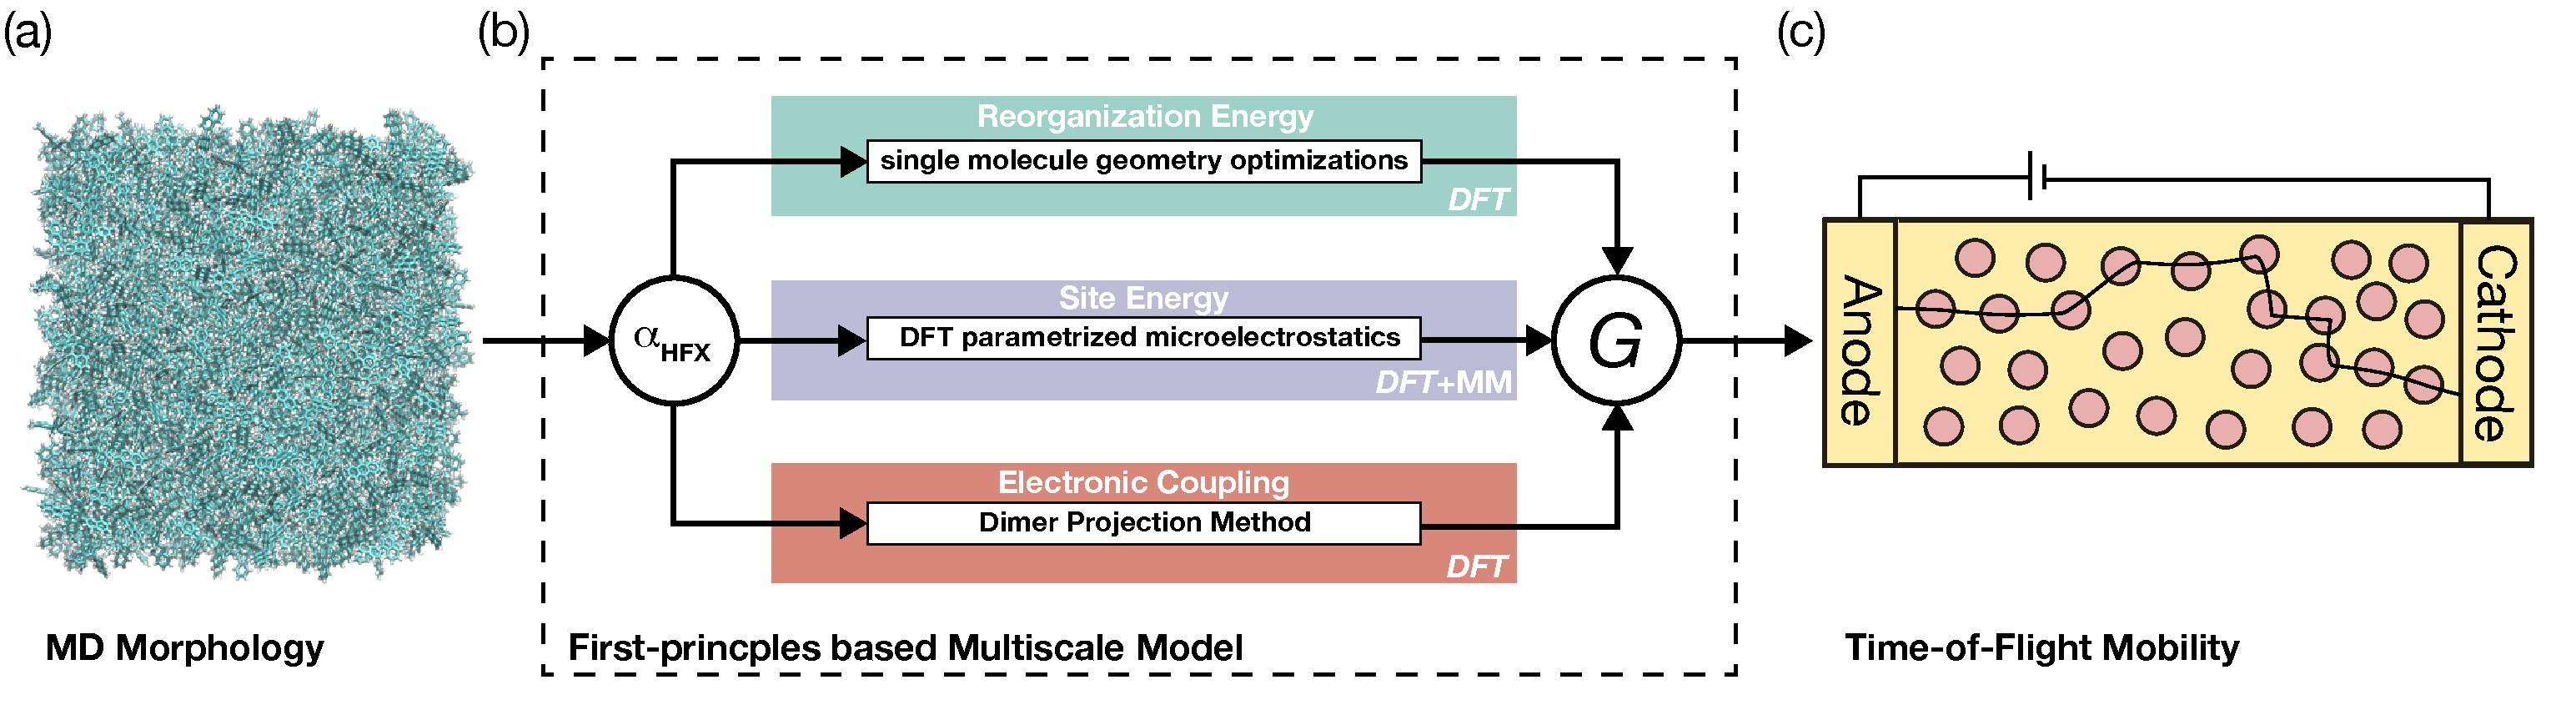
\includegraphics[width=\linewidth]{figs/MSM2.pdf}
  \caption{\bjoern{TODO Bjoern}{Rewrite caption}The multiscale model workflow for OSC. Step 1: MD simulation to generate atom coordinates. Step 2: Molecule energy $E_i$ calculation. Step 3: Calculation of Reorganization energy $\lambda_{ij}$ and coupling element $J_{ij}$ for pairs of molecule $i,j$ whose COM distance is less than $r_\text{cutoff}$. Step 4: Modelling dynamics on device level, such as ToF calculation.}
  \label{fig:MSM}
\end{figure*}

Fundamentally, quantum-mechanical description is needed to model charge dynamics due to the motion of electrons. However, the resulting full many-electron schr\"{o}dinger equation is impossible to solve due to its complexity, so Density Functional Theory (DFT) \cite{kohn_selfconsistent_1965,jones_density_2015, hammesschiffer_conundrum_2017} appears as a manageable way to model electrons.
DFT has its own challenges in achieving multiscale modeling.
The first challenge relates to the Born-Oppenheimer approximation \cite{born_zur_1927} in quantum
mechanics, which simplifies the problem by separating the electronic and nuclear
coordinates. As a result, the time evolution of the atomic coordinates can be modeled in molecular dynamics (MD) by solving the Newton's equation using empirical force field to approximate the potential energy surfaces~\cite{rapaport_art_2004}. 

The next challenge is the infeasibility of solving the DFT equations for the entire system even at a fixed time~\cite{hammesschiffer_conundrum_2017}. 
But due to fact that OSCs have disordered and amorphous structure and the quantum states of each molecule is confined to a limited region, the charge dynamic can be well-approxmiated as a jumping process between molecules, which is a continuous time random walk (CTRW) process.
The transition rates between the molecules can be calculated from quantum chemical calculations and related to the electronic structures parameters including the molecule energy, reorganization energy and coupling elements which will be explained in the methodology section. 


Until this point, the molecular system is modeled as graph $\mathbf{G}(\mathbf{V}, \mathbf{W})$ where $\mathbf{V}$ is the set of nodes and $\mathbf{W}: \omega_{ij}$ is the adjacency matrix. Each node represents one molecule, the weighted and directed edge $\omega_{ij}$ represents the transition rates from node $i$ to node $j$ calculated from quantum chemical methods. 
As will be shown in the method section, $\omega_{ij}$ determines the QoIs whose quantities we want to quantify.

Figure \ref{fig:MSM} summarized the multiscale model as mentioned above using MADN, a type of OSC as an example. 
The process includes: Firstly, classical Molecular Dynamics is used to generate the atomistic coordinates of all molecules. Then DFT is used to obtain electronic structures. Finally the charge dynamic is model as a CTRW among the molecules.

\bjoern{Uncertainties in the MSM}{way too verbose}
In achieving the multiscale model, uncertainties are introduced. 
While Born-Oppenheimer approximation allows for the use of force field to approximate the potential energy surfaces and model the atomic coordinates using Newton’s equations, the force field is not exactly the same as the potential for DFT~\cite{izvekov_effective_2004}. 
So the atomic coordinates, that is the molecule structures contain uncertainty which ultimately affects the charge dynamics. 
This is one source of uncertainty that have not been investigated. But in our investigation, a fixed molecule structure is used and we do not consider this source of uncertainty. 
Secondly, charge jumping between the state localization is not exactly a time dependent DFT process. 
However, the amorphous OSCs used in this work has strong disorder, so the model noise from state localization is negligible and we do not consider the uncertainty originated from this perspective.

\bjoern{Focus on functional dependence}{should talk about the sensitivity of the functional first, then say that looking at HFX is a 'single-parameter' study.} Lastly, the source of uncertain that this work focus on comes from the approximation for the exchange-correlation energy in DFT. 
There is no exact formula for the exchange-correlation functional, so in practical approximations are developed and tested to guarantee the robustness of DFT method~\cite{gunnarsson_exchange_1976, bilc_hybrid_2008, lee_development_1988}. 
The accuracy of DFT depends heavily on the choice of the exchange-correlation functional whose suitability is usually unknown for new synthesized molecules. 
As an advancement to improve accuracy, Hybrid-DFT \cite{marques_densitybased_2011,perdew_rationale_1996} incorporates a portion $\alpha$ of exact HF exchange functional (HFX) from Hartree-Fock (HF) theory into the exchange-correlation functional, particularly for systems where DFT falls short. For example, the PBE0 functional has a portion of 0.25 HFX~\cite{adamo_toward_1999}.

Looking back into the CTRW of the charge transport, the transition rates depend on the electronic structures parameters which rely on the validity of the exchange-correlation functional from the modeling perspectives.
So the approximations in exchange-correlation functional will bring uncertainties to the multiscale model~\cite{medvedev_density_2017}. 
In particular, different hybrid-DFT functionals containing varying HFX levels will generate different output from the multiscale model mentioned aboved. 
The effect of such uncertainty from the electronic structure level on the multiscale model is not yet explored in literatures. 
The goal of this work is to quantify the uncertainty effect of the exchange-correlation functional on the charge dynamics in OSCs and to study the robustness of the multiscale model, with a particular focus on the uncertainty represented by different portional of HFX.

\bjoern{Definition of a QoI}{is ToF (mobility)} A QoI need be chosen to perform this goal of uncertainty quantification. 
The figure of merit in OSC investigation is the charge mobility, which quantitatively describe how fast charges move in an OSC. 
The charge mobility is commonly measured in a \textit{time-of-flight} (ToF) setting. 
As shown in Fig.\ref{fig:MSM}(d), charge carriers are injected into one electrode called \textit{Source} and they are collected by another electrode at the opposite end called \textit{Sink}. 
Knowing the length of the sample $L$ and the time-of-flight $\tau$, the diffusive velocity is calculated as $v_\text{ToF}=\frac{L}{\tau}$.
When electric field $\vec{F}$ is used and the charge dynamics undergo a field-drifted transport, the charge mobility is calculated as $\mu_\text{ToF}=\frac{\vec{v}_\text{ToF} \vec{F}}{|\vec{F}|^2}$. 

%Some literatures also report a steady state setting for investigation of charge mobility. In such condition, there is no \textit{Source}-\textit{Sink} boundary condition. Instead, the molecular system is infinitely repeated in all three dimensions by periodic boundary conditions. 
%Over a long time period, the charge occupation on each molecule $\pi_i$ reach an equilibrium, allowing a steady state distribution to be obtained.
%The steady state charge velocity $v_\text{SS}$ is calculated as the charge velocity along the direction of the electric field normalized by the steady state charge occupation $\vec{\pi}:\pi_i$. 
%The calculation for $v_\text{ToF}$ and $\mu_\text{SS}$ will be detailed in the method section.

\bjoern{Rephrase}{!}To quantify the uncertainty for QoI, the focus of our work will be placed on answering the following questions: 
\begin{enumerate}
    \item How does HFX level change the electronic structures: reorganization energy, distribution of molecule energies and coupling elements? 
    \item How does HFX level change the charge mobility?
    \item Which electronic structure (among energy, coupling element and reorganization energy) uncertainty has the most impact on the QoI distribution?
    \item Can we estimate the range of the QoI, given a confidence level?
\end{enumerate}

\bjoern{Update}{later} The rest of the paper is organized as follows. Section 2 will outline the multiscale model in OSCs. This includes the electronic structure calculation centering on Kohn-Sham equation, the calucation of molecule energy, reorganization energy and coupling elements. The details of the molecule dynamics to obtain the MADN system will be listed.
Then section 3 present the multiscale modeling results with the chosen HFX values. In section 4, the Monte Carlo sampling method is utilized to estimate the ToF distribution and $v_\text{SS}$ distribution, followed by the sensitivity analysis on the parameters. 
Section 5 shows calculated Poole-Frankel behavior of the MADN with varying HFX values. The confidence interval of the Poole-Frankel plot is estimated. Section 6 concludes the paper. 

\section{Multiscale Model}
As mentioned in the introduction, the multiscale model maps a structural morphology into a graph $\mathbf{G}(\mathbf{V}, \mathbf{W})$. In our context, the graph properties, that is the entries $\omega_{ij}$ in the adjacency matrix $\mathbf{W}$, only depends on the HFX values since other modeling parameters are kept consistent. 

Those transition rates charge transfer rates from molecules $i$ to $j$ is calculated as the bi-molecular transition rates:
%
\begin{equation}
    \omega_{ij} = \frac{2\pi}{\hbar} \frac{|J_{ij}|^2}{\sqrt{4\pi \lambda_{ij} k_\text{B}T}} \exp\left(-\frac{(E_{ij} + q \vec{F} \cdot \vec{r}_{ij} - \lambda_{ij})^2}{4\lambda_{ij} k_\text{B}T}\right) ,
    \label{equ:Marcus}
\end{equation}
%
where $\hbar$ is the reduced Planck constant and $k_\text{B}$ the Boltzmann constant. The temperature $T$ (in \unit[]{K}), the charge of the carrier $q$ (in \unit[]{e}) and the external electric field $\vec{F}$ (in V/m) can be considered the external, environmental parameters of the simulation. The vector $\vec{r}_{ij} = (r^x_{ij},r^y_{ij},r^z_{ij})^\text{T}$ connects the center-of-masses (COMs) of molecules $i$ and $j$, which is calculated using cyclic boundary conditions. 
The remaining physical, material-specific (or rather transfer-pair-specific) quantities are the reorganization energy $\lambda_{ij}$, the electronic coupling $J_{ij}$, and the energy difference $E_{ij} = E_i - E_j$ (all in \unit[]{eV}). 
In our model, two nodes $i,j$ form a connection of the corresponding molecules $i,j$ have their closest-contact distance smaller than $r_\text{cutoff}=\unit[0.5]{nm}$.
The rest of this section will introduce the following: the molecular dynamics used to obtain the coordinates $r^x_{i},r^y_{i},r^z_{i}$, the calculation of node-specific quantities $\lambda$, $E_i$ and $J_{ij}$, as well as the calculation of ToF $\tau$ and steady state velocity $v_\text{SS}$.

%%%%%%%%%%%%%%%%%%%%%%%%%%%%%%%%%%%%%%%%%%%%%%%%%%%%%%%%%
\subsection{Molecular Dynamics}
The OSC morphology, that is the spacial coordinate of all the atoms, are generated by molecule dynamics. The GROMACS software package~\cite{berendsen_gromacs_1995} is utilized to implement atomistic molecular dynamics simulations of bulk amorphous MADN with the empirical force field obtained via Automated Topology Builder~\cite{stroet_automated_2018}.

The MADN system starts with 1000 MADN molecules randomly placed in a cubic cell with a large enougth side length to allow a low density. Periodic boundary conditions are applied throughout in all three spatial directions. After energy minimization, the system is simulated for \unit[1]{ns} (?) in a $NpT$ ensemble, keeping a constant temperature of \unit[300]{K} and constant pressure of \unit[1]{bar} using the V-rescale thermostat~\cite{bussi_canonical_2007} with the coupling time constant \unit[0.1]{ps} and the Parrinello-Rahman barostat~\cite{parrinello_polymorphic_1981} with a time constant for pressure coupling \unit[2]{ps}. 
The equation of motion for updating the atomic coordinates is implemented by leap-frog algorithm~\cite{van_gunsteren_leap} with a time step of \unit[1]{fs}. 

Following this, simulated annealing is applied to relax the MADN.  
The temperature is increased to \unit[800]{K}, well above the glass transition temperature during a period of \unit[0.5]{ns}. 
This temperature is maintained for \unit[1]{ns} before cooling back down to \unit[300]{K} during a period of \unit[0.5]{ns}.
Such heating-cooling cycle is repeated three times. After this simulated annealing, a production run is conducted for \unit[2]{ns} using the $NpT$ ensemble. The final configuration of MADN is chosen for the further steps in the multiscale model, whose configuration is a cubic box with a length of \unit[9.0]{nm} and a density of $\unit[1.08]{g/cm^3}$. 
%%%%%%%%%%%%%%%%%%%%%%%%%%%%%%%%%%%%%%%%%%%%%%%%%%%%%%%%%%%%%%%

\subsection{Electronic Structure Calculations} 
\label{sec:es}
Starting from an atomic morphology, a first step in first-principle multiscale model is to determine the single-electronic wave function and the associated energy $\epsilon_l$, which are used to obtain atomic charges, reorganization energy, molecule energy, and coupling elements.

Each electron $l$ in a system with $N_\text{el}$ electrons has a single-electronic wave function $\phi_l (\vec{r})$ and associated energies $\epsilon_l$ determined as solutions to the Kohn--Sham equations~\cite{kohn_self_1965}
%
\begin{eqnarray}
    && \left(-\frac{1}{2}\nabla^2_{\vec{r}} + v_\text{ext}(\vec{r}) + v_\text{H}[\rho](\vec{r}) + v_\text{XC}[\rho](\vec{r})\right) \phi_l(\vec{r}) \nonumber \\
    && = H^\text{KS} \phi_l(\vec{r}) = \epsilon_l \phi_l (\vec{r}) ,
    \label{eq:KS2}
\end{eqnarray}
%
where $v_\text{ext}$ in an external potential (typically from the nuclei), $v_\text{H}[\rho]$ the electrostatic Hartree potential of a classical charge density $\rho(\vec{r})$, and $v_\text{XC}[\rho]$ the exchange-correlation functional containing explicit quantum-mechanical electron-electron interactions. The charge density is determined from the single-particle wave functions as $\rho(\vec{r})=\sum\limits_{l=1}^{N_\text{el}} \left\vert\phi_l(\vec{r})\right\vert^2$. As the Hartree and exchange-correlation potential depend on the thus defined density, solutions to Eq.~\ref{eq:KS2} have to be found self-consistently. This corresponds to finding the ground-state density $\rho_0$ that minimized the total energy of the system
%
\begin{equation}
    U[\rho] = T_s[\rho] + \int v_\text{ext}(\vec{r}) \rho(\vec{r}) d \vec{r} + E_\text{H}[\rho] + E_\text{XC}[\rho]
    \label{eq:KS_model}
\end{equation}
%
where $T_s[\rho]$ is the kinetic energy, $E_\text{H}[\rho]$ and $E_\text{XC}[\rho]$ the Hartree and exchange-correlation energies, respectively. 

The practical calculations in this work have been performed with the ORCA software~\cite{Neese2012a} using the def2-tzvp~\cite{weigend_accurate_2006} basis set to represent the Kohn--Sham wave functions $\phi_l(\vec{r})$. 
The correlation potential is represented by PBE0 functional, and the exchange potential is represented by a portion $\alpha$ of (HFX) potential and another portion $(1-\alpha)$ from PBE0 functional. In common practice, $\alpha$ is small and below 0.25. For our uncertain quantification study, $\alpha=0,0.05,0.10,0.15,0.20,0.25$ is chosen for the multiscale model.

\subsection{Transition Rate Calculation}
Electronic structure calculation via Equation \ref{eq:KS2} and \ref{eq:KS_model} are performed for different combinations of molecular charge states $x=$ n,c and the corresponding equilibrium geometries $X=$ N,C. The notion n and N stand for "neutral", and the notion c and C stand for "charged". 
Following this, the total energy will be denoted as $U^\text{xX}$, dropping of the explicit functional dependency on the density $\rho$. 
The reorganization energy $\lambda$ accounts for the energy change caused by the geometry variation during the charge transport, and is linked to the total energy via:
%
\begin{equation}
    \lambda_{ij} = U_i^\text{nC} - U_i^\text{nN} + U_j^\text{cN} - U_j^\text{cC}
    \label{eq:lambda}
\end{equation}
%
In this work, the OSC only has one type of molecule, and $\lambda_{ij}$ of all molecular pairs are equal. So the subscript is left out and denoted as $\lambda$.

The molecule energy $E_i = E_i^\text{c} - E_i^\text{n}$ is the difference between the total energies of the system in which molecule $i$ is carrying a charge or not, corresponding to the ionization potential in case of hole transport and the negative of the electron affinity in case of electron transport. 

These total energies in turn consist of different contributions associated with different physical mechanism, i.e.,
%
\begin{equation}
E_i^x = U_i^{xX} + E_i^{x,\text{el}} + E_i^{x,\text{polar}},
\label{eq:Es}
\end{equation}
%
where $U_i^{xX}$ is the internal energy from single molecules as above.
Both $E_i^{x,\text{el}}$ and $E_i^{x,\text{polar}}$ are contributions arising from intermolecular interactions: $E_i^{x,\text{el}}$ is the electrostatic energy due to the surrounding molecules and $E_i^{x,\text{polar}}$ is the polarization energy. 
These contributions are calculated with a microelectrostatic model using parametrized point charge representations\cite{https://doi.org/10.1002/jcc.540110311}

In the multiscale model, $E_i^{x,\text{el}}$ is evaluated with a \unit[4]{nm} cutoff distance:
%
\begin{equation}
    E_i^{x,\text{el}} = \frac{1}{4 \pi \epsilon_0} \sum\limits_{a_i} \sum\limits_{b_k,k \neq i} \frac{(q^c_{a_i} - q^n_{b_i})q^n_{b_k}}{ r_{a_i b_k}} 
\end{equation}
%
where $\epsilon_0$ is the vacuum permittivity, $a_i, b_k$ denotes the atoms in molecule $i,k$, $q^{n(c)}_{a_i}$ are the partial charge of atom $a$ when molecule $i$ is in state x. And $r_{a_i b_k} = |r_{a_i} - r_{b_k}|$ is the distance between atoms $a_i$ and $b_k$, which should be within \unit[4]{nm} due to the cutoff setting. 
For the purpose of quantifying uncertainty in HFX, the long-range electrostatic interactions are not considered. 

The polarization effects are determined self-consistently to consider the response of the molecules to the associated fields~\cite{thole_molecular_1981}.
Polarization effects are considered in a region of \unit[4.0]{nm} around each individual molecule. Practical calculations of the site energies are performed using the VOTCA software~\cite{Baumeier2011,doi:10.1021/acs.jctc.8b00617,10.1063/1.5144277,Baumeier2024}.


The coupling element $J_{ij}$ between molecule $i$ and $j$ describe the coupling strength between two localized states. In the case of hole transport, the relevant orbitals are highest-occupied molecular orbital (HOMO) of the isolated molecules (monomers) $\phi^\text{HOMO}_i(\vec{r})$ and $\phi^\text{HOMO}_j(\vec{r})$, 
leading to the calculation of $J_{ij}$ is implemented using the Dimer-Projection Method~\cite{baumeier_density_2010}. Specifically, the coupling element is determined as:
Specifically, the coupling element is determined as: 
%
\begin{equation}
    J_{ij} = \frac{ J^0_{ij}- \frac{1}{2}(e_i+e_j) S_{ij} }{ 1- S_{ij}^2 }
    \label{equ:JAB}
\end{equation}
%
where $J^0_{ij} = \langle \phi^\text{HOMO}_i | \hat{H}^\text{KS}_\text{D} | \phi^\text{HOMO}_j \rangle $, $e_i = \langle \phi^\text{HOMO}_i | \hat{H}^\text{KS}_\text{D} | \phi^\text{HOMO}_i \rangle $, $e_j = \langle \phi^\text{HOMO}_j | \hat{H}^\text{KS}_\text{D} | \phi^\text{HOMO}_j \rangle $, and $S_{ij}=\langle \phi^\text{HOMO}_i | \phi^\text{HOMO}_j \rangle $ with bra-ket notation. 
and $H^\text{KS}_\text{D}$ is the Hamiltonian of the dimer (see Eq.~\ref{eq:KS2}). 
As the Hamiltonian of the dimer is diagonal in its eigenbasis $\left\{ \phi_\text{D}(\vec{r})\right\}$ with eigenvalues $\left\{ \epsilon_D\right\}$, so $H^\text{KS}_\text{D} = \text{diag}(\epsilon_D)$, $J^0_{ij}$ can be calculated as $J^0_{ij} = \mathbf{p}_i^\text{T} \text{diag}(\epsilon_\text{D}) \mathbf{p}_j$,  where the vector $\mathbf{p}_i = \langle \phi_i^\text{HOMO} | \phi^\text{HOMO}_\text{D} \rangle$ and $\mathbf{p}_j = \langle \phi_j^\text{HOMO} | \phi_\text{D}^\text{HOMO} \rangle$ are the projections of the monomer orbitals $\phi_i^\text{HOMO}, \phi_j^\text{HOMO}$ onto the dimer orbitals $\phi^\text{HOMO}_\text{D}$. Similarly, $e_{i(j)} = \mathbf{p}_{i(j)}^\text{T} \mathbf{p}_{i(j)}$ and $S_{ij} =  \mathbf{p}_i^\text{T} \mathbf{p}_j$. All  of these operations are performed in the basis set representation of the Kohn--Sham wave functions (see Sec.~\ref{sec:es}) as implemented in VOTCA.

\subsection{Time-of-flight and Steady State Velocity Calculation}
Following the graph $\mathbf{G}$ from the multiscale model,
The charge dynamics are modeled as a continuous-time random walk on this graph. In the time-of-flight (ToF) model, some vertices serve as \textit{Source} nodes, representing the electrode where charge carriers are injected, and some as \textit{Sink} nodes, where charge carriers are detected and the ToF is recorded.
In CTRW the ToF is calculated as the expected hitting time of a continuous time Markov chain.
For a system with $N$ molecules and one charge carriers, there are $N$ possible occupation states. A state is called the Source state if one of the Source molecule is occupied, and a Sink state is the one when one of the Sink molecule is occupied.

The transition rates between the states define the adjacency matrix $\mathbf{W}:\omega_{ij}$.
According to such connectivity between the molecules, the transition rates $\mathbf{W}_{ij}$ from state $i$ to $j$ is:
%
\begin{equation}
  \label{eq:transition_rates}
	\mathbf{W}_{ij} =
	\begin{cases}
	     0			&  i \text{ is not connected to } j,\\
         \omega_{ij}   &  i \text{ is connected to } j,
	\end{cases}
\end{equation}

Then the transition probability from state $i$ to $j$ is $p_{ij} = \mathbf{W}_{ij}/D_i$ where $D_i := \sum_{j} \mathbf{W}_{ij}$.
And the expected time from state $i$ to reach the Sink state $\tau_i$ is calculated via: 
%
\begin{equation}
  \label{eq:hitting_time}
	\tau_i = \begin{cases}
		\frac{1}{D_i} + \sum_{j \ne i} p_{ij} \tau_{j} &\text{if $i$ is not a sink state},\\
		0 &\text{else.} 
	\end{cases}
\end{equation} 

To account for all possible starting nodes of the carriers, all Source states must be considered. The random walk process can be modeled as a parallel electric network of capacitors~\cite{doyle_random_1984}. Accordingly, the ToF is evaluated using the harmonic mean:
%
\begin{equation} 
  \tau = N_\text{source} \left[\sum_{i \in \text{Source}} (\tau_i)^{-1}\right]^{-1},
  \label{eq:ToF}
\end{equation}
%
where $N_\text{source}$ is the number of Source states.

%To calculate $v_\text{SS}$ the steady state distribution $\pi_i$ is required. In continuous time Markov chain, the steady state distribution vector $\vec{\pi}: \pi_i$ is the null-space of $\mathbf{W}-\mathbf{D}$:
%\begin{equation}
%    (\mathbf{W}-\mathbf{D} )\vec{\pi} = \mathbf{0}
%\end{equation}
%where $\mathbf{D} = \text{diag}(D_i)$ is the out-degree matrix of $\mathbf{W}$.

%\begin{equation}
%    v_\text{SS} = \sum_i \pi_i \sum_j \omega_{ij} || \vec{r}_{ij}||_2
%\end{equation} 
%where $\omega_{ij}$ is the charge transition rate from molecule $i$ to molecule $j$, and $\vec{r}_{ij}=\vec{r}_j - \vec{r}_i$ is the center-of-mass (COM) distance vector. 
%%%%%%%%%%%%%%%%%%%%%%%%%%%%%%%%%%%%%%%%%%%%%%%%%%%%%%%%%%

\section{Results on MADN}

In this study, we investigate the hole-transporting organic semiconductor MADN (2-Methyl-9,10-di(naphth-2-yl)anthracene) and study its charge mobility's dependence on HFX. 

Atomic charges and molecule polarizability $P_\text{iso}$ are crucial for evaluating molecular energy contributions from electrostatic and polarization effects. A physical property related to the overall atomic charges is dipole moment at charge neutral state. 


\begin{figure}[tbp]
    \centering
    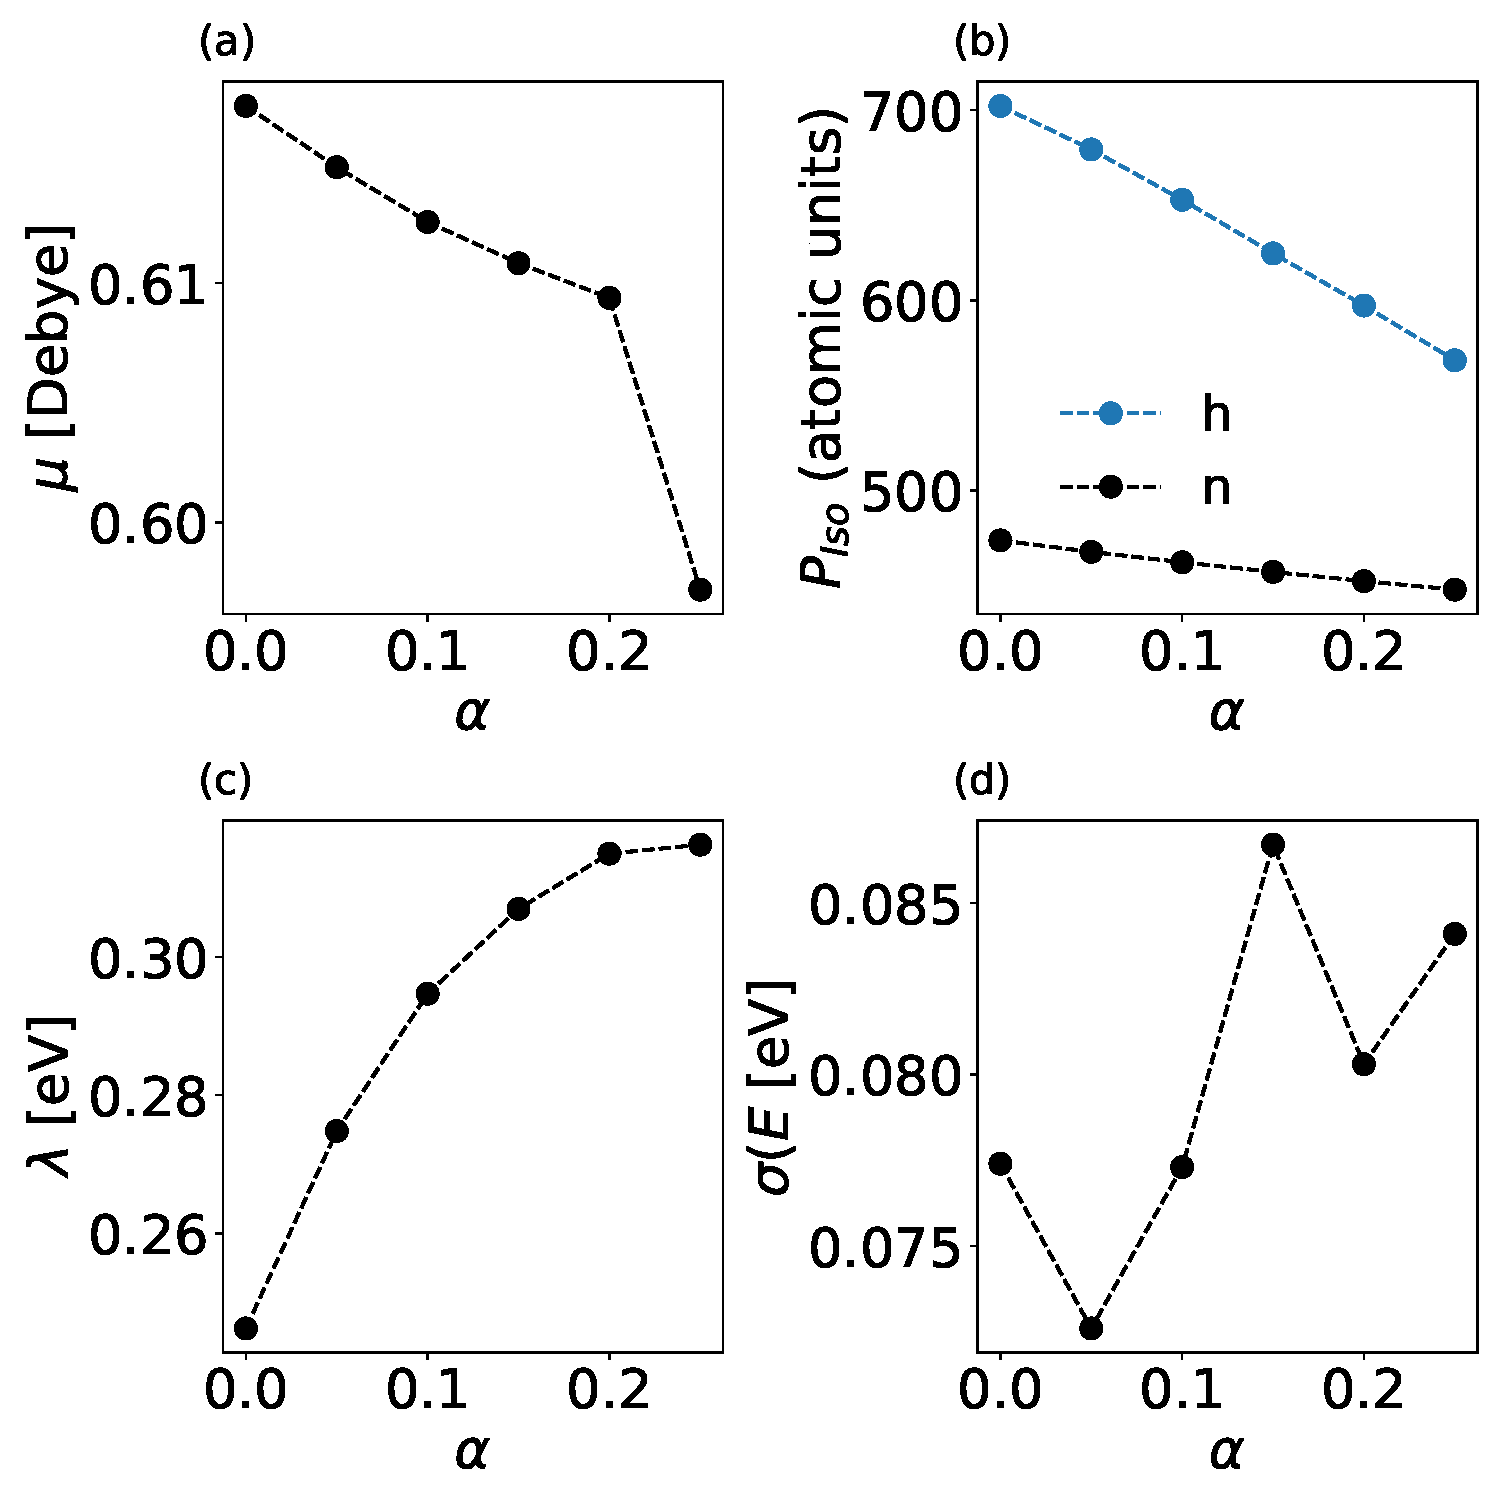
\includegraphics[width=\linewidth]{figs/fig_autogen.pdf}
    \caption{\bjoern{TODO Zhong:}{The labels (a), (b), (c),(d) should be bigger and places at slightly to the left from the individual panels, which includes the y axis labels; panel (b): these atomic units can be abbreviated a.u. and you should also use [a.u.] and not round brackets; pane (d) is missing a ); I would also like to use $\alpha_{HF}$ throughout the paper; change $\mu$ to $d$.}(a) The dipole moment of neutral state MAND molecule $\mu$, (b) isotropic polarizability $P_\text{iso}$, (c) reorganization energies $\lambda$ and (d) energy disorder $\sigma(E)$ as a function of the HFX parameters (denoted by $\alpha$).}
    \label{fig:autogen_MADN}
\end{figure}


To demonstration the effect of HFX on the atomic charges and molecule polarizability $P_\text{iso}$,
Figure \ref{fig:autogen_MADN}(a)(b) illustrates the dependence of the dipole moment $\mu$ and isotropic polarizability $P_\text{iso}$ on HFX.
Figure \ref{fig:autogen_MADN}(c)(d) show 
The reorganization energy $\lambda$ and energy disorder $\sigma(E)$ as a function of HFX parameter are also shown in Fig.~\ref{fig:autogen_MADN}(c)(d).

From Fig.~\ref{fig:autogen_MADN}(a) one can notice a mild decrease in the dipole moment with increasing HFX and in Fig.~\ref{fig:autogen_MADN}(b) a linear decrease in isotropic polarizability for both neutral and charged MADN states as HFX increases from 0 to 0.25, indicating reduced molecular polarizability.
Figure~\ref{fig:autogen_MADN}(c) indicates an increase in reorganization energy $\lambda$ with higher HFX, reflecting greater energy requirements for electronic adjustments during charge transfer. This increase is nonlinear compared to the linear decrease in $P_\text{iso}$.
Figure~\ref{fig:autogen_MADN}(d) shows that the energy disorder $\sigma(E)$ for MADN are similar and close to \unit[0.08]{eV} under different HFX values.

To calculate the ToF from the electronic structures, the \textit{Source} region contains molecules with X-coordinate $0 < r^x_i < 0.5$ nm, and the \textit{Sink} region contains molecules with X-coordinate $8.5 < r^x_i < 9$ nm. 

The ToF is also calculated without energy disorder, meaning $\Delta E_{ij}=0$ for all $i,j$.
Table \ref{tab:ToF_MADN_HFX} shows the ToF and corresponding diffusive velocity $v_\text{ToF}$.
With energy disorder, the ToF increases by a factor of approximately 15 as $\alpha$ increases from 0 to 0.25.  
While without energy disorder, the increase factor is about 4. This increase in ToF is attributed to the rise in $\lambda$, changes in molecular energies, and variations in coupling elements.

\begin{table}[tbp]%The best place to locate the table environment is directly after its first reference in text
\caption{\label{tab:ToF_MADN_HFX}%
The ToF and diffusive velocity calculated by ToF along a distance $L_x = \unit[9.0]{nm}$ with and without energy disorder of the MADN system as a function of the HFX. The ToF is in unit $\unit[]{s}$ and $v_\text{ToF}$ in unit $\unit[]{m/s}$.
}
\begin{ruledtabular}
  \begin{tabular}{c c c c c}
        $\alpha$ & ToF& $v_\text{ToF}$ & ToF(no $E$)& $v_\text{ToF}$(no $E$) \\
    \hline
        0.00 &  $6.4 \times 10^{-9}$ & 1.2 & $1.9 \times 10^{-10}$ & 42 \\
        0.05 & $ 7.9 \times 10^{-9}$ & 1.0 & $4.1 \times 10^{-10}$ & 20 \\
        0.10 & $ 1.6 \times 10^{-8}$ & 0.51 & $4.0 \times 10^{-10} $ & 20 \\
        0.15 & $ 3.0 \times 10^{-8}$ & 0.31 & $4.0 \times 10^{-10} $ & 25 \\
        0.20 & $ 2.1 \times 10^{-8}$ & 0.39 & $4.5 \times 10^{-10}$ & 18 \\
        0.25 & $ 9.5 \times 10^{-8}$ & 0.083 & $7.2 \times 10^{-10}$ & 11 \\
    \end{tabular}
\end{ruledtabular}
\end{table}

%
\begin{table*}[tbp]%The best place to locate the table environment is directly after its first reference in text
\caption{\label{tab:W2_E}%
The 1-Wasserstein distance between the distributions pair of molecule energy $P_{E(\alpha)}$, electrostatic energy $P_{E^\text{el}(\alpha)}$, polar energy $P_{E^\text{polar}(\alpha)}$ and $P_{\log_{10}(J_{ij}^2)(\alpha)}$.
}
\begin{ruledtabular}
  \begin{tabular}{c c c c c c}
  $\alpha'$ & 0 & 0.05 & 0.10 & 0.15 & 0.20 \\
    \hline
  $W_1 (P_{E(\alpha')}, P_{E(\alpha=0.25)})$ &  0.0054 & 0.0091 & 0.0067 & 0.0053 & 0.0045 \\
  $W_1 (P_{E^\text{el}(\alpha')}, P_{E^\text{el}(\alpha=0.25)})$ &  0.010 & 0.012 & 0.0089 & 0.0070 & 0.0032 \\
  $W_1 (P_{E^\text{polar}(\alpha')}, P_{E^\text{polar}(\alpha=0.25)})$ &  0.0065 & 0.0043 & 0.0027 & 0.0023 & 0.0031 \\
  $W_1 (P_{\log_{10}(J_{ij}^2)(\alpha')}, P_{\log_{10}(J_{ij}^2)(\alpha=0.25)})$ &  0.0054 & 0.0091 & 0.0067 & 0.0053 & 0.0045 \\
    \end{tabular}
\end{ruledtabular}
\end{table*}
%
  
\begin{figure*}
  \centering
  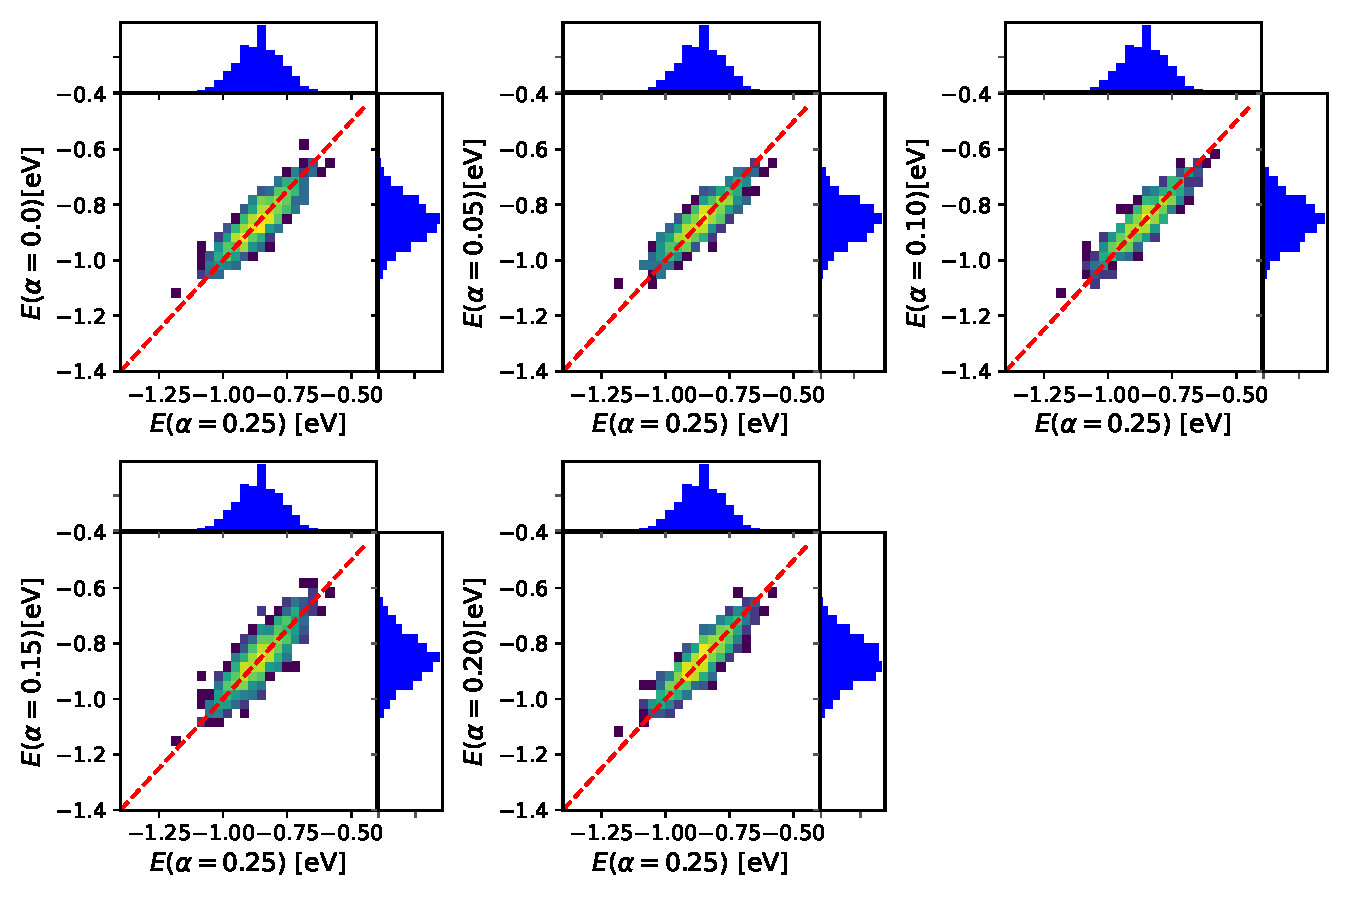
\includegraphics[width=0.80\textwidth]{figs/scatterE_qmmm.pdf}
  \caption{\bjoern{TODO Zhong:}{add labels (a)...; replace $\alpha$ with $\alpha_\text{HF}$.}Scatter plot of site energy of MADN molecules calculated from different HFX, compared to the site energy calculated from HFX=0.25 (The PBE0 functional). The brighter color near the diagonal lines indicates denser population of the molecules.  The top and right histogram show the energy distributions.}
  \label{fig:E_qmmm_MADN}
\end{figure*}

\begin{figure*}
  \centering
  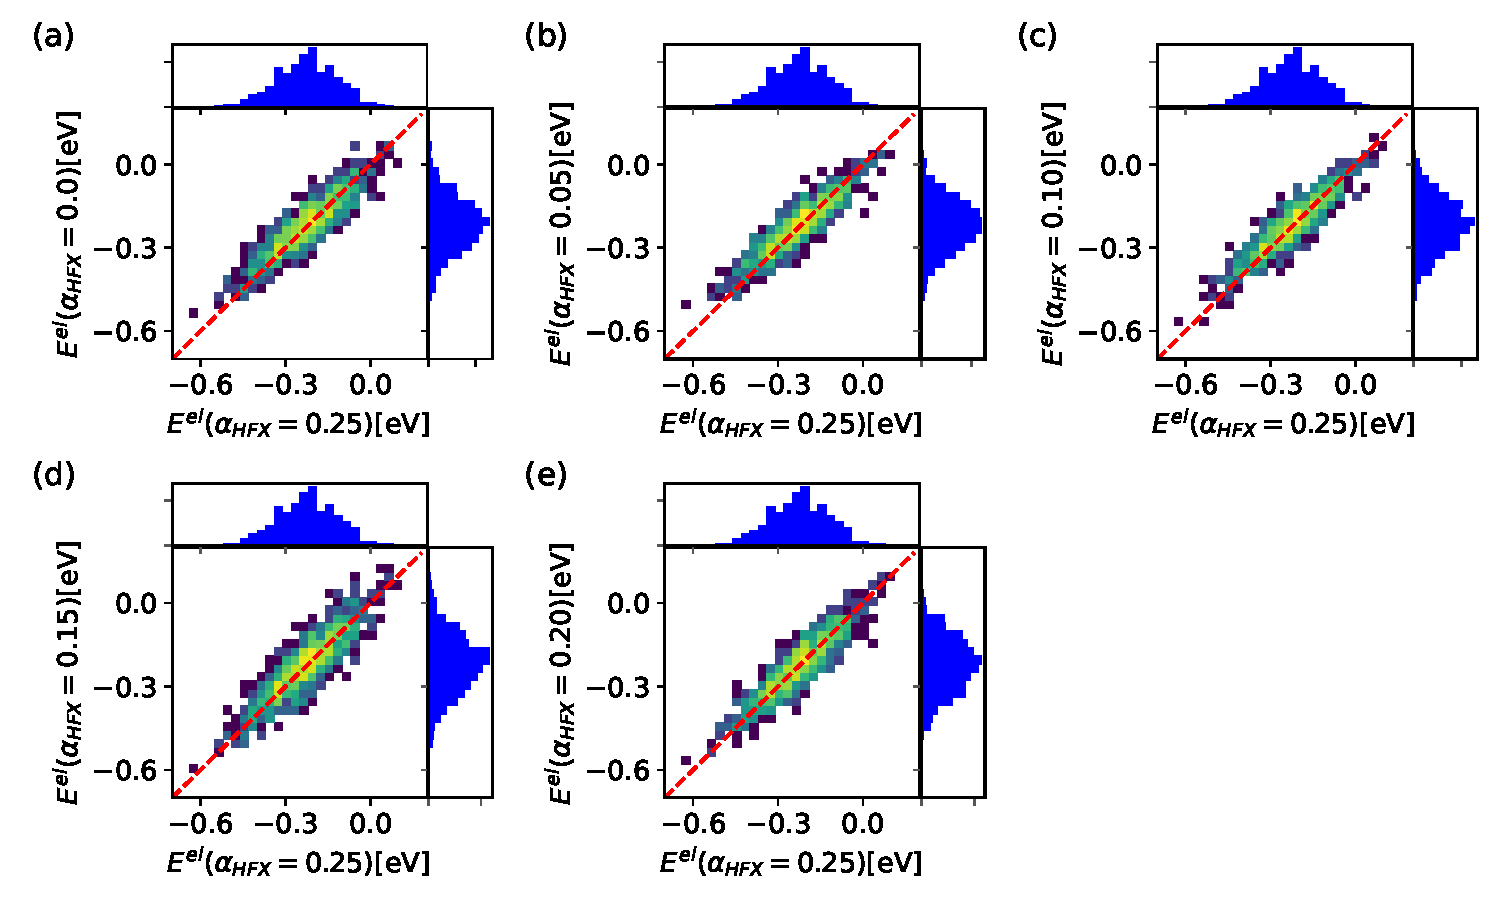
\includegraphics[width=0.80\textwidth]{figs/scatterEstat_qmmm.pdf}
  \caption{\bjoern{TODO Zhong:}{add labels (a)...; replace $\alpha$ with $\alpha_\text{HF}$.}Scatter plot of MADN electrostatic energy calculated from different HFX, compared to the electrostatic energy calculated from HFX=0.25 (The PBE0 functional). The brighter color near the diagonal lines indicates denser population of the molecules.  The top and right histogram show the energy distributions.}
  \label{fig:Estat_qmmm_MADN}
\end{figure*}

\begin{figure*}
  \centering
  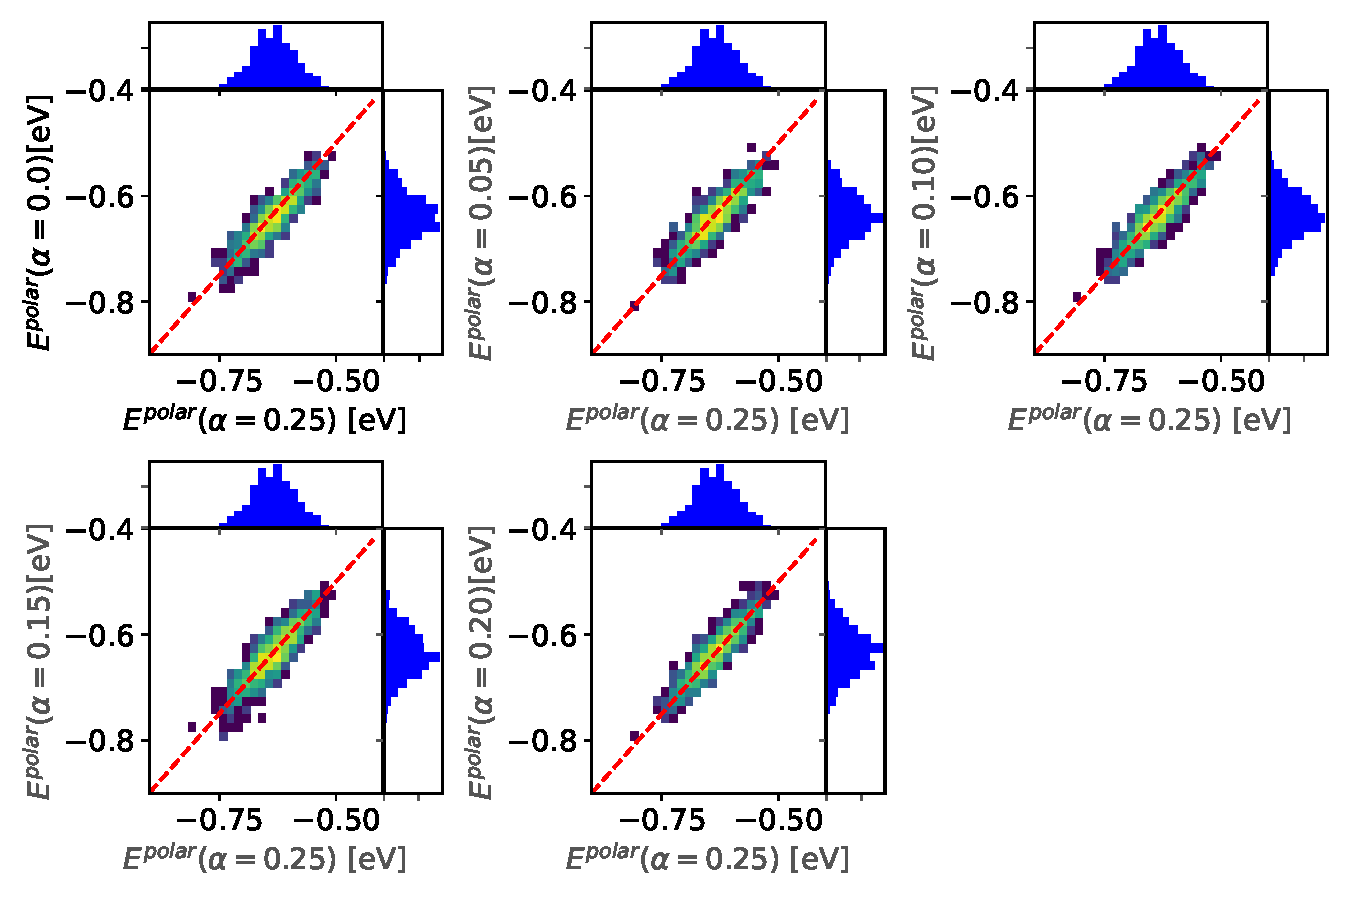
\includegraphics[width=0.80\textwidth]{figs/scatterEdip_qmmm.pdf}
  \caption{\bjoern{TODO Zhong:}{add labels (a)...; replace $\alpha$ with $\alpha_\text{HF}$.}Scatter plot of MADN polarization energy calculated from different HFX, compared to the polarization energy calculated from HFX=0.25 (The PBE0 functional). The brighter color near the diagonal lines indicates denser population of the molecules.  The top and right histogram show the energy distributions.}
  \label{fig:Edip_qmmm_MADN}
\end{figure*}

\begin{figure*}
  \centering
  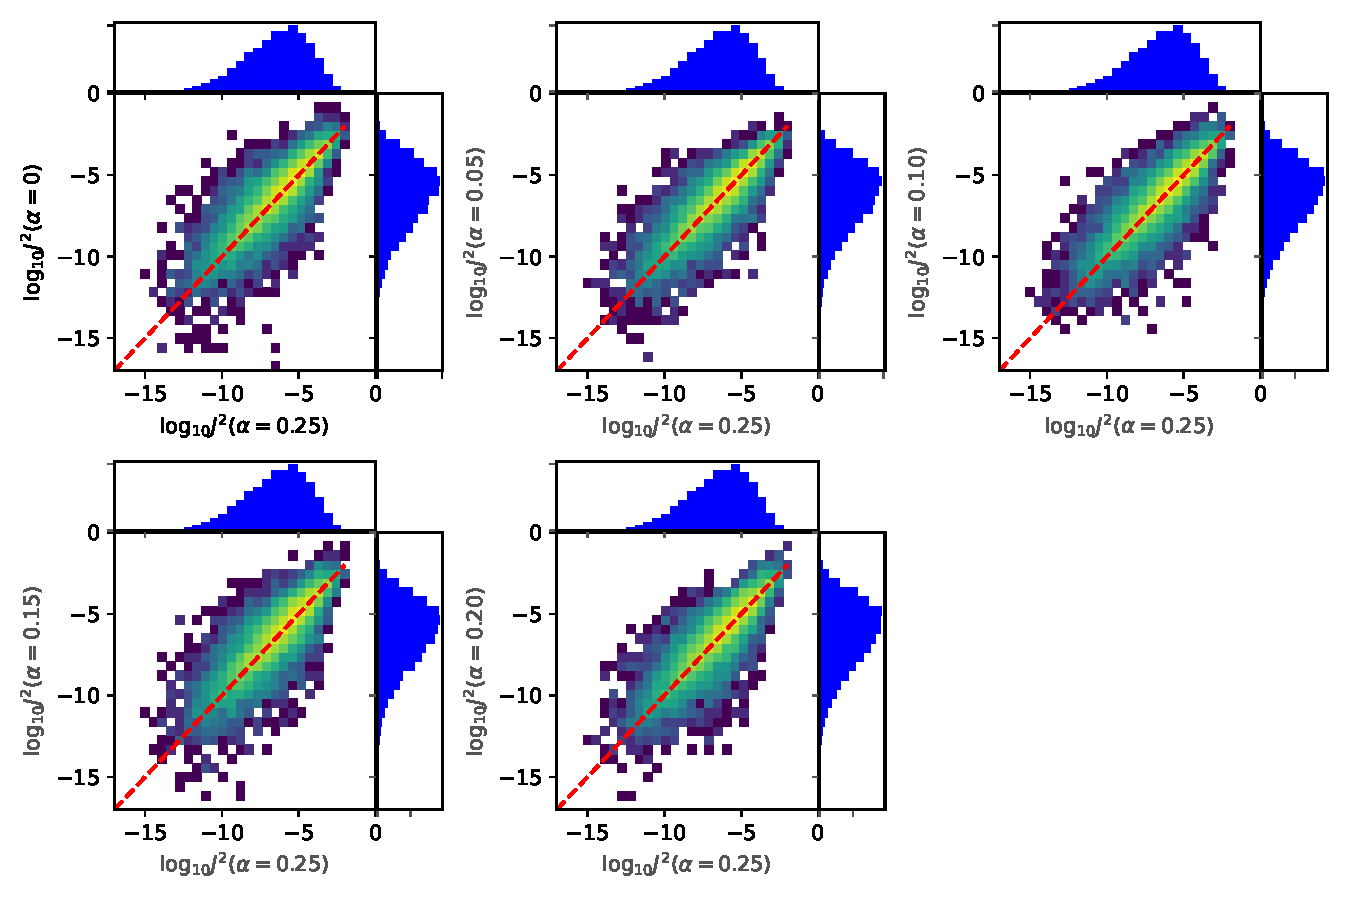
\includegraphics[width=0.80\textwidth]{figs/scatterJ_all.pdf}
  \caption{\bjoern{TODO Zhong:}{add labels (a)...; replace $\alpha$ with $\alpha_\text{HF}$; it should be $\log_{10}(J^2/(\unit[]{eV})^2)$; make sure the 10 of $\log_{10}$ is not touching $J$.} Scatter plot of MADN coupling element $\log_{10} J^2$ calculated from different HFX, compared to the polarization energy calculated from HFX=0.25 (The PBE0 functional). The brighter color near the diagonal lines indicates denser population of the molecules.  The top and right histogram show the energy distributions.}
  \label{fig:J_MADN}
\end{figure*}

Figure \ref{fig:E_qmmm_MADN} presents a scatter plot comparing the site energies of MADN molecules across different HFX values, using $\alpha$ = 0.25 (PBE0 functional) as a reference for which the calculated molecule energy has a range from -1.17 to -0.60 \unit[]{eV}y.
The range of molecule energy for the other five HFX are: 
from -1.11 to -0.59 \unit[]{eV} for $\alpha=0$, 
from -1.07 to -0.63 \unit[]{eV} for $\alpha=0.05$, 
from -1.13 to -0.61 \unit[]{eV} for $\alpha=0.10$
from -1.16 to -0.60 \unit[]{eV} for $\alpha=0.15$, 
and from -1.12 to -0.63 \unit[]{eV} for $\alpha=0.20$.
The bright-yellow color in all plots of Fig. \ref{fig:E_qmmm_MADN} indicates that most data points are clustering near the diagonal line, so the molecular energies calculated by different HFX are very close.

To quantify the similarity between two empirical distribution, Wasserstein distance~\cite{villani_optimal_2009} is used.
Denote the empirical distribution of molecular energy $E$ at $\alpha=0$ to be $P_{E(\alpha=0)}$. 
The 1-Wasserstein distance between $P_{E(\alpha=0)}$ and $P_{E(\alpha=0.25)}$ is calculated as:
\begin{eqnarray}
    && W_1 (P_{E(\alpha=0)}, P_{E(\alpha=0.25)}) = \nonumber \\
    && \frac{1}{N} \sum\limits_{i=1}^N | E_{(i)}(\alpha=0) - E_{(i)}(\alpha=0.25) |
\end{eqnarray}
where $E_{(i)}(\alpha=0)$ is the order statistics of $E_i(\alpha=0)$. The 1-Wasserstein distance between two empirical distributions for each plot in Fig. \ref{fig:E_qmmm_MADN} is shown in Table \ref{tab:W2_E}. $W_1 (P_{E(\alpha=0)}, P_{E(\alpha=0.25)})$ has range between 0.0045 to 0.0091, indicating that the molecular energy distributions are very similar. 


To further estimate the energy variation due to HFX, one can look at the molecule that has maximum $|E_i(\alpha=0.25) - E_i(\alpha')|$ for all molecule index $i=1,2,\cdots,N$. 
This quantity provides information of the amount of the largest variation one can expect in $E_i(\alpha)$. Index the molecule that has maximum $|E_i(\alpha=0.25) - E_i(\alpha')|$ to be $i'$. 
If molecule $i'$ energy is the lowest one among the $N$ molecules, then a further change (such as lowering) in the energy of molecule $i'$ may lead to large change in ToF, since low energy potentially lead to a trap in the charge transport dynamics and significantly affects the mobility. 

Table \ref{tab:maxEi} shows that depending on $\alpha'$, the maximum $|E_i(\alpha=0.25) - E_i(\alpha')|$ is 0.12 to 0.15, which is considerable small compared to the range of molecular energy and the magnitude of the energy disorder, which is around 0.08 as shown in Fig. \ref{fig:autogen_MADN}. 
The energy of molecule $i'$ shown in Table \ref{tab:maxEi} indicates that the $i'$ molecule energy is not the lowest one in the system. So the maximum energy variation quantified by $\max(|E_i(\alpha=0.25) - E_i(\alpha')|)$ is not likely to results in large change in ToF due to trapping effects. 
%
\begin{table}[tbp]%The best place to locate the table environment is directly after its first reference in text
\caption{\label{tab:maxEi}%
In the tested $\alpha'$ values, the second column shows the maximum of $E_i(\alpha=0.25) - E_i(\alpha')$ for all molecules. Denoting $i'$ as the index of the molecule which has maximum $E_i(\alpha=0.25) - E_i(\alpha')$ for the chosen $\alpha'$, the third column shows the energy of molecule $i'$ calculated by $\alpha=0.25$. The fourth column shows the molecule energy $E_{i'}(\alpha')$ calculated by $\alpha'$. All the energies are in unit $\unit[]{eV}$.
}
\begin{ruledtabular}
  \begin{tabular}{c c c c}
  $\alpha'$ & $\max(|E_i(\alpha=0.25) - E_i(\alpha')|)$  & $E_{i'}(\alpha=0.25)$ & $E_{i'}(\alpha')$ \\
    \hline
  0 & 0.13 &  -1.07 & -0.94 \\
  0.05 & 0.12 & -0.82 & -0.94 \\
  0.10 & 0.13 & -1.07 & -0.94 \\
  0.15 & 0.15 & -0.84 & -0.69 \\
  0.20 & 0.12 & -0.70 & -0.82 \\
    \end{tabular}
\end{ruledtabular}
\end{table}

Figures \ref{fig:Estat_qmmm_MADN} and \ref{fig:Edip_qmmm_MADN} show that both electrostatic and polarization energies remain consistently close to the ones calculated from $\alpha=0.25$, since all the points comparing $E^\text{el}_i(\alpha')$ and $E^\text{el}_i(\alpha=0.25)$ in the scatter plot are close to the diagonal line.
The range of $E^\text{el}$ calculated by different $\alpha$ is as follows:
from  -0.55 to 0.078 eV for $\alpha=0$, 
from  -0.52 to 0.047 eV for $\alpha=0.05$, 
from  -0.57 to 0.086 eV for $\alpha=0.10$, 
from  -0.59 to 0.14 eV for $\alpha=0.15$, 
from  -0.57 to 0.10 eV for $\alpha=0.20$, 
and from -0.63 to 0.10 eV for $\alpha=0.25$.


The 1-Wasserstein distance between the distribution of $E^\text{el}$ calculated by $\alpha'$ and that calculated by $\alpha=0.25$, $W_1(P_{E^\text{el}(\alpha')}, P_{E^\text{el}(\alpha=0.25)})$, is shown at the third row at Table \ref{tab:W2_E}. 
The maximum of $W_1(P_{E^\text{el}(\alpha')}, P_{E^\text{el}(\alpha=0.25)})$ 0.012. The 1-Wasserstein distance between the $E^\text{polar}$ distribution calculated by $\alpha'$ and that calculated by $\alpha=0.25$ is also shown in Table \ref{tab:W2_E}, with a maximum of 0.006. So the small Wasserstein distances suggest that the using different $\alpha'$ other than $\alpha=0.25$, the data of $E, E^\text{el}, E^\text{polar}$ have not changed significantly.

The standard deviations of the electrostatic energy are 0.099, 0.094, 0.099, 0.11, 0.10, \unit[0.10]{eV}, and the standard deviations of the polarization energies are 0.044, 0.043, 0.043, 0.047, 0.045, \unit[0.045]{eV}. So the disorder in electrostatic energies is consistently larger than that in molecule energies, and the palorization effect reduces the electrostatic energy disorder. 
Each individual molecule has similar polarization energies under different HFX calculation, in spite of $P_\text{iso}$ is linearly dependent on HFX. 

The coupling element obtained with different HFX for each molecular pair compared to that obtained with HFX=0.25 is shown in the scatter plot Fig. \ref{fig:J_MADN}.


The distribution of the majority $\log_{10} J_{ij}^2$ has a range of -14 to -2 while only a few $\log_{10} J_{ij}^2$ has low value below -15. For all HFX values, the distribution has a peak at around -5. 
For large values $\log_{10} J_{ij}^2 < -5$ the coupling element calculated from $\alpha'=0, 0.05, 0.10, 0.15, 0.2$ remains consistently close to that calculated by $\alpha=0.25$. While for small values $\log_{10} J_{ij}^2 > -5$, the $\alpha'$ calculated coupling elements for a specific molecular pair can have large variation compared to $\log_{10} J_{ij}^2$ calculated using $\alpha=0.25$.
The 1-Wasserstein distance between the $J$ distributions obtained by different $\alpha$ is always smaller than 0.01,  
indicating similar $J$ distributions even though a few $J_{ij}$ shows large difference when $\alpha$ varies. 

In charge transport network, $J_{ij}^2$ is undirectional for a molecular pair, and decays exponentially as the mutual center-of-mass distance increases. The large $\log_{10} J_{ij}^2$ are usually observed when molecular $i$ and $j$ are close.
When the center-of-mass distance is very large, the $\log_{10} J_{ij}^2$ is small and some of those small $\log_{10} J_{ij}^2$ are sensitive to $\alpha$. 

However, the charge dynamics is dominated by large $\log_{10} J_{ij}^2$ which are found between molecule pair having small center-of-mass. As the center-of-mass distance increases, $\log_{10} J^2$ becomes small and negligible for the charge dynamics. So the small $J_{ij}$ may not have noticeable effect on the ToF although their calculated values from different HFX are very different. 

To determine the range of $\log_{10} J^2$ that are significant for the charge dynamics, a percolation algorithm is performed. This algorithm aims to find the largest size of subgraphs after removing the edges whose coupling elements are below a critical value. The procedure is as follows:
\begin{enumerate}
    \item A critical value $J_c$ is chosen,
    \item In graph $\mathbf{G}$ remove all the edges with $J_{ij}^2 < J_c^2$
    \item Calculate the maximum size $\max({N_\text{sub}})$ of the connected subgraphs
\end{enumerate}

\begin{figure}[btp]
  \centering
  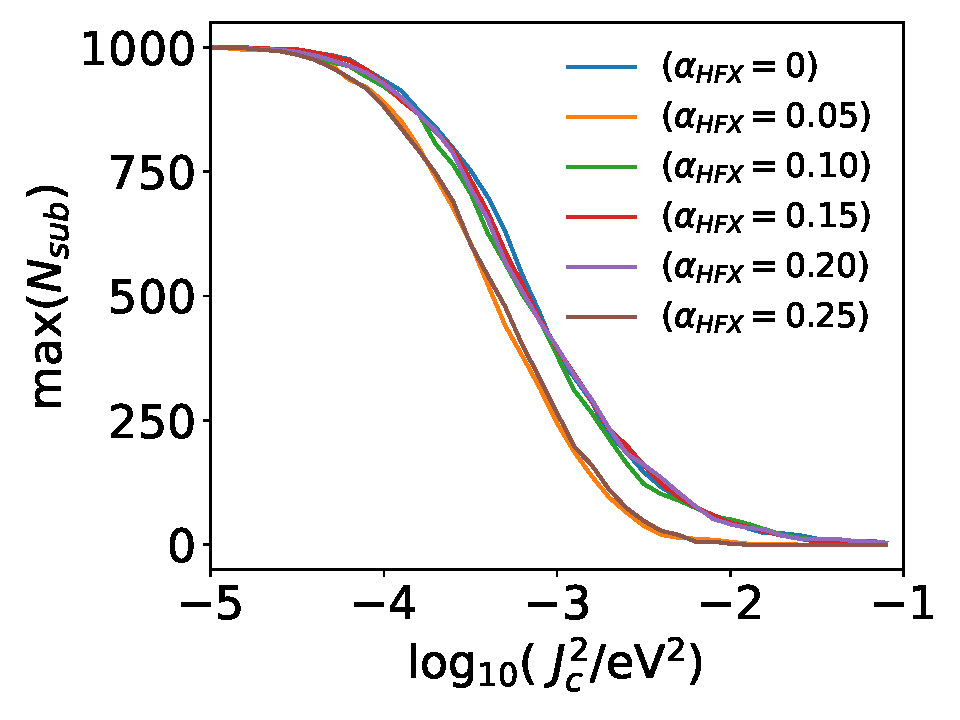
\includegraphics[width=0.45\textwidth]{figs/fig_network_all.pdf}
  \caption{\bjoern{TODO Zhong:}{same comments regarding the $\log_{10}$ as above; replace $\alpha$ with $\alpha_\text{HF}$.}The maximum size of the subgraphs obtained in the percolation algorithm as a function of critical value $J_c$. The molecular systems obtained by different HFX are colored according to the legend.}
  \label{fig:J_percolate}
\end{figure}

\begin{table}[t]
  \caption{\label{tab:ToF_J} The ToF along a distance $L_x = 9 \unit[]{nm}$  of the MADN system as a function of the HFX. The molecular connections with coupling element $\log_{10} J^2_{ij} < 5$ are deleted.}
  \centering
  \begin{tabular}{c c c c }
  \hline
  \hline
      $\alpha$ & & & ToF [s]  \\
  \hline
      0.00 & & &  $7.5 \times 10^{-9}$ \\
      0.05 & & & $ 8.1 \times 10^{-9}$ \\
      0.10 & & & $ 1.6 \times 10^{-8}$ \\
      0.15 & & & $ 3.1 \times 10^{-8}$ \\
      0.20 & & & $ 2.5 \times 10^{-8}$ \\
      0.25 & & & $ 9.7 \times 10^{-8}$ \\
  \hline
  \hline
  \end{tabular}
\end{table}

After performing percolation algorithm, Figure \ref{fig:J_percolate} shows the dependence of $\max({N_\text{sub}})$ on the critical value $J_c$. When $\log_{10} J_c^2 < 5$, $\max({N_\text{sub}})$ is 1000, meaning that removing all the edges with $J_{ij}^2 < 1 \times 10^{-5}$ the 1000 vertexes still form a connected graph. 
But when removing the edges with $J_{ij}^2 < 3.1 \times 10^{-4}$ ( corresponding to $J_c > -3.5$), the maximum size subgraph is 600, and it quickly decreases as $J_c$ increases, showing a phase transition. 
So the dominated coupling elements are those with $\log_{10} J_c^2 > -5$. 
And the variation in small $J_{ij}$ due to HFX has less impact on the charge dynamics. Table \ref{tab:ToF_J} shows the ToF for the MADN system after deleting the molecular connections with  $\log_{10} J_c^2 < -5$. The resulting ToF is close to the values obtained without deleting any connections (shown in Table \ref{tab:ToF_MADN_HFX}).
The increase of ToF after deleting the connections with  $\log_{10} J_c^2 < -5$ is always less than 30\%, confirming that the molecular connections with the small $J_{ij}$ has small effect in ToF. 

In this section we answer the question of how does HF level change the electronic structures ($\lambda, E_i, J_{ij}$) and 
how does HF level change the ToF. 
In the next section, uncertainty quantification via Monte Carlo method and sensitivity analysis is performed to answer which electronic structure (among energy, coupling element and reorganization energy) uncertainty has the most impact on the ToF distribution. 
And further we estimate the range of the quantity of interest, given a confidence level.
%%%%%%%%%%%%%%%%%%%%%%%%%%%%%%%%%%%%%%%%%%%%%%%%%%%%%%%%%

\section{ToF Distribution and Sensitivity Analysis}
The previous section shows that different HFX affect the calculated ToF. In this section, we use the Monte Carlo method to estimate the range of the ToF given a confidence level, followed by a sensitivity analysis to determine which parameter contributes more to the variance of ToF. 

\subsection{ToF Distribution}
The ToF is calculated from electronic structure ($E$, $\lambda$ and $\log_{10}(J^2)$) data, that is, ToF is a function with the input of all electronic structure parameters:
\begin{equation}
    %\tau = g(\lambda, \{E_i|i=1,2,\cdots,N \}, \{J_{ij}|i,j=1,2,\cdots,N \}) \;
    \tau = g(x_1, x_2, \cdots, x_{N_d})
    \label{eq:tau1}
\end{equation}
The input $(x_1, x_2, \cdots, x_{N_d})$ represents the collection of the parameters $$(\lambda, \{E_i|i=1,2,\cdots,N \}, \{J_{ij}|i,j=1,2,\cdots,N \})$$  where $N_d$ is the parameter dimension, that is the number of input parameters. 
And $\{E_i|i=1,2,\cdots,N \}$ is the ordered set whose elements are the molecule energy,
$\{J_{ij}|i,j=1,2,\cdots,N \}$ is the ordered set whose elements are the coupling elements. 

Each parameter has uncertainty caused by the exchange-correlation functional in the multiscale model.
To estimate the uncertainty which is unknown, we consider the maximum amount of uncertainties according to the obtained $(\lambda, \{E_i|i=1,2,\cdots,N \}, \{J_{ij}|i,j=1,2,\cdots,N \})$ with the six different HFX.
To achieve this, each parameter can be modeled as a normal distribution with the mean and standard deviation obtained by the maximum likelihood estimation. For a normal distribution, they are respectively the sample mean and standard deviation obtained by six different HFXs.

Then Monte Carlo scheme is used to estimate the distribution of the ToF. The Monte Carlo scheme has the procedure:
\begin{enumerate}
\item For all $i,j=1,2,\cdots, N_d$, obtain a realization $(x_1, x_2, \cdots, x_{N_d})$ where each parameter has the normal distribution, meaning the corresponding electronic parameters are sampled from the distribution $\lambda_i \in \mathcal{N}(\mathbb{E}(\lambda), \mathbb{V}(\lambda))$, $E_i \in \mathcal{N}(\mathbb{E}(E_i), \mathbb{V}(E_i))$, $\log_{10}(J_{ij}^2) \in \mathcal{N}(\mathbb{E}(\log_{10}(J_{ij}^2)), \mathbb{V}(\log_{10}(J_{ij}^2)))$. 
\item Calculate ToF using the sampled data set $(x_1, x_2, \cdots, x_{Nd})$. 
\item Repeat step 1 and 2 for $N_\text{MC} = 50000$ times to obtain ToFs. Plot the distribution of the ToFs.
\item Estimate the 99\% confidence interval around the median.
\end{enumerate}


To understand how the uncertainty pass from $E, \lambda, J_{ij}$ to ToF, the parameter control is used. That is, a set of parameter, such as $E_i$ for all $i=1,2,\cdots,N$ is choose while keeping other parameter fixed, then performed Monte Carlo sampling to obtain ToF distribution and estimate upper and lower confidence bound.
Then we use Sobol total indices to analyze and quantify 
which uncertainty among $E, \lambda, J_{ij}$ has a greater impact on the ToF, 

%
\begin{figure}
  \centering
  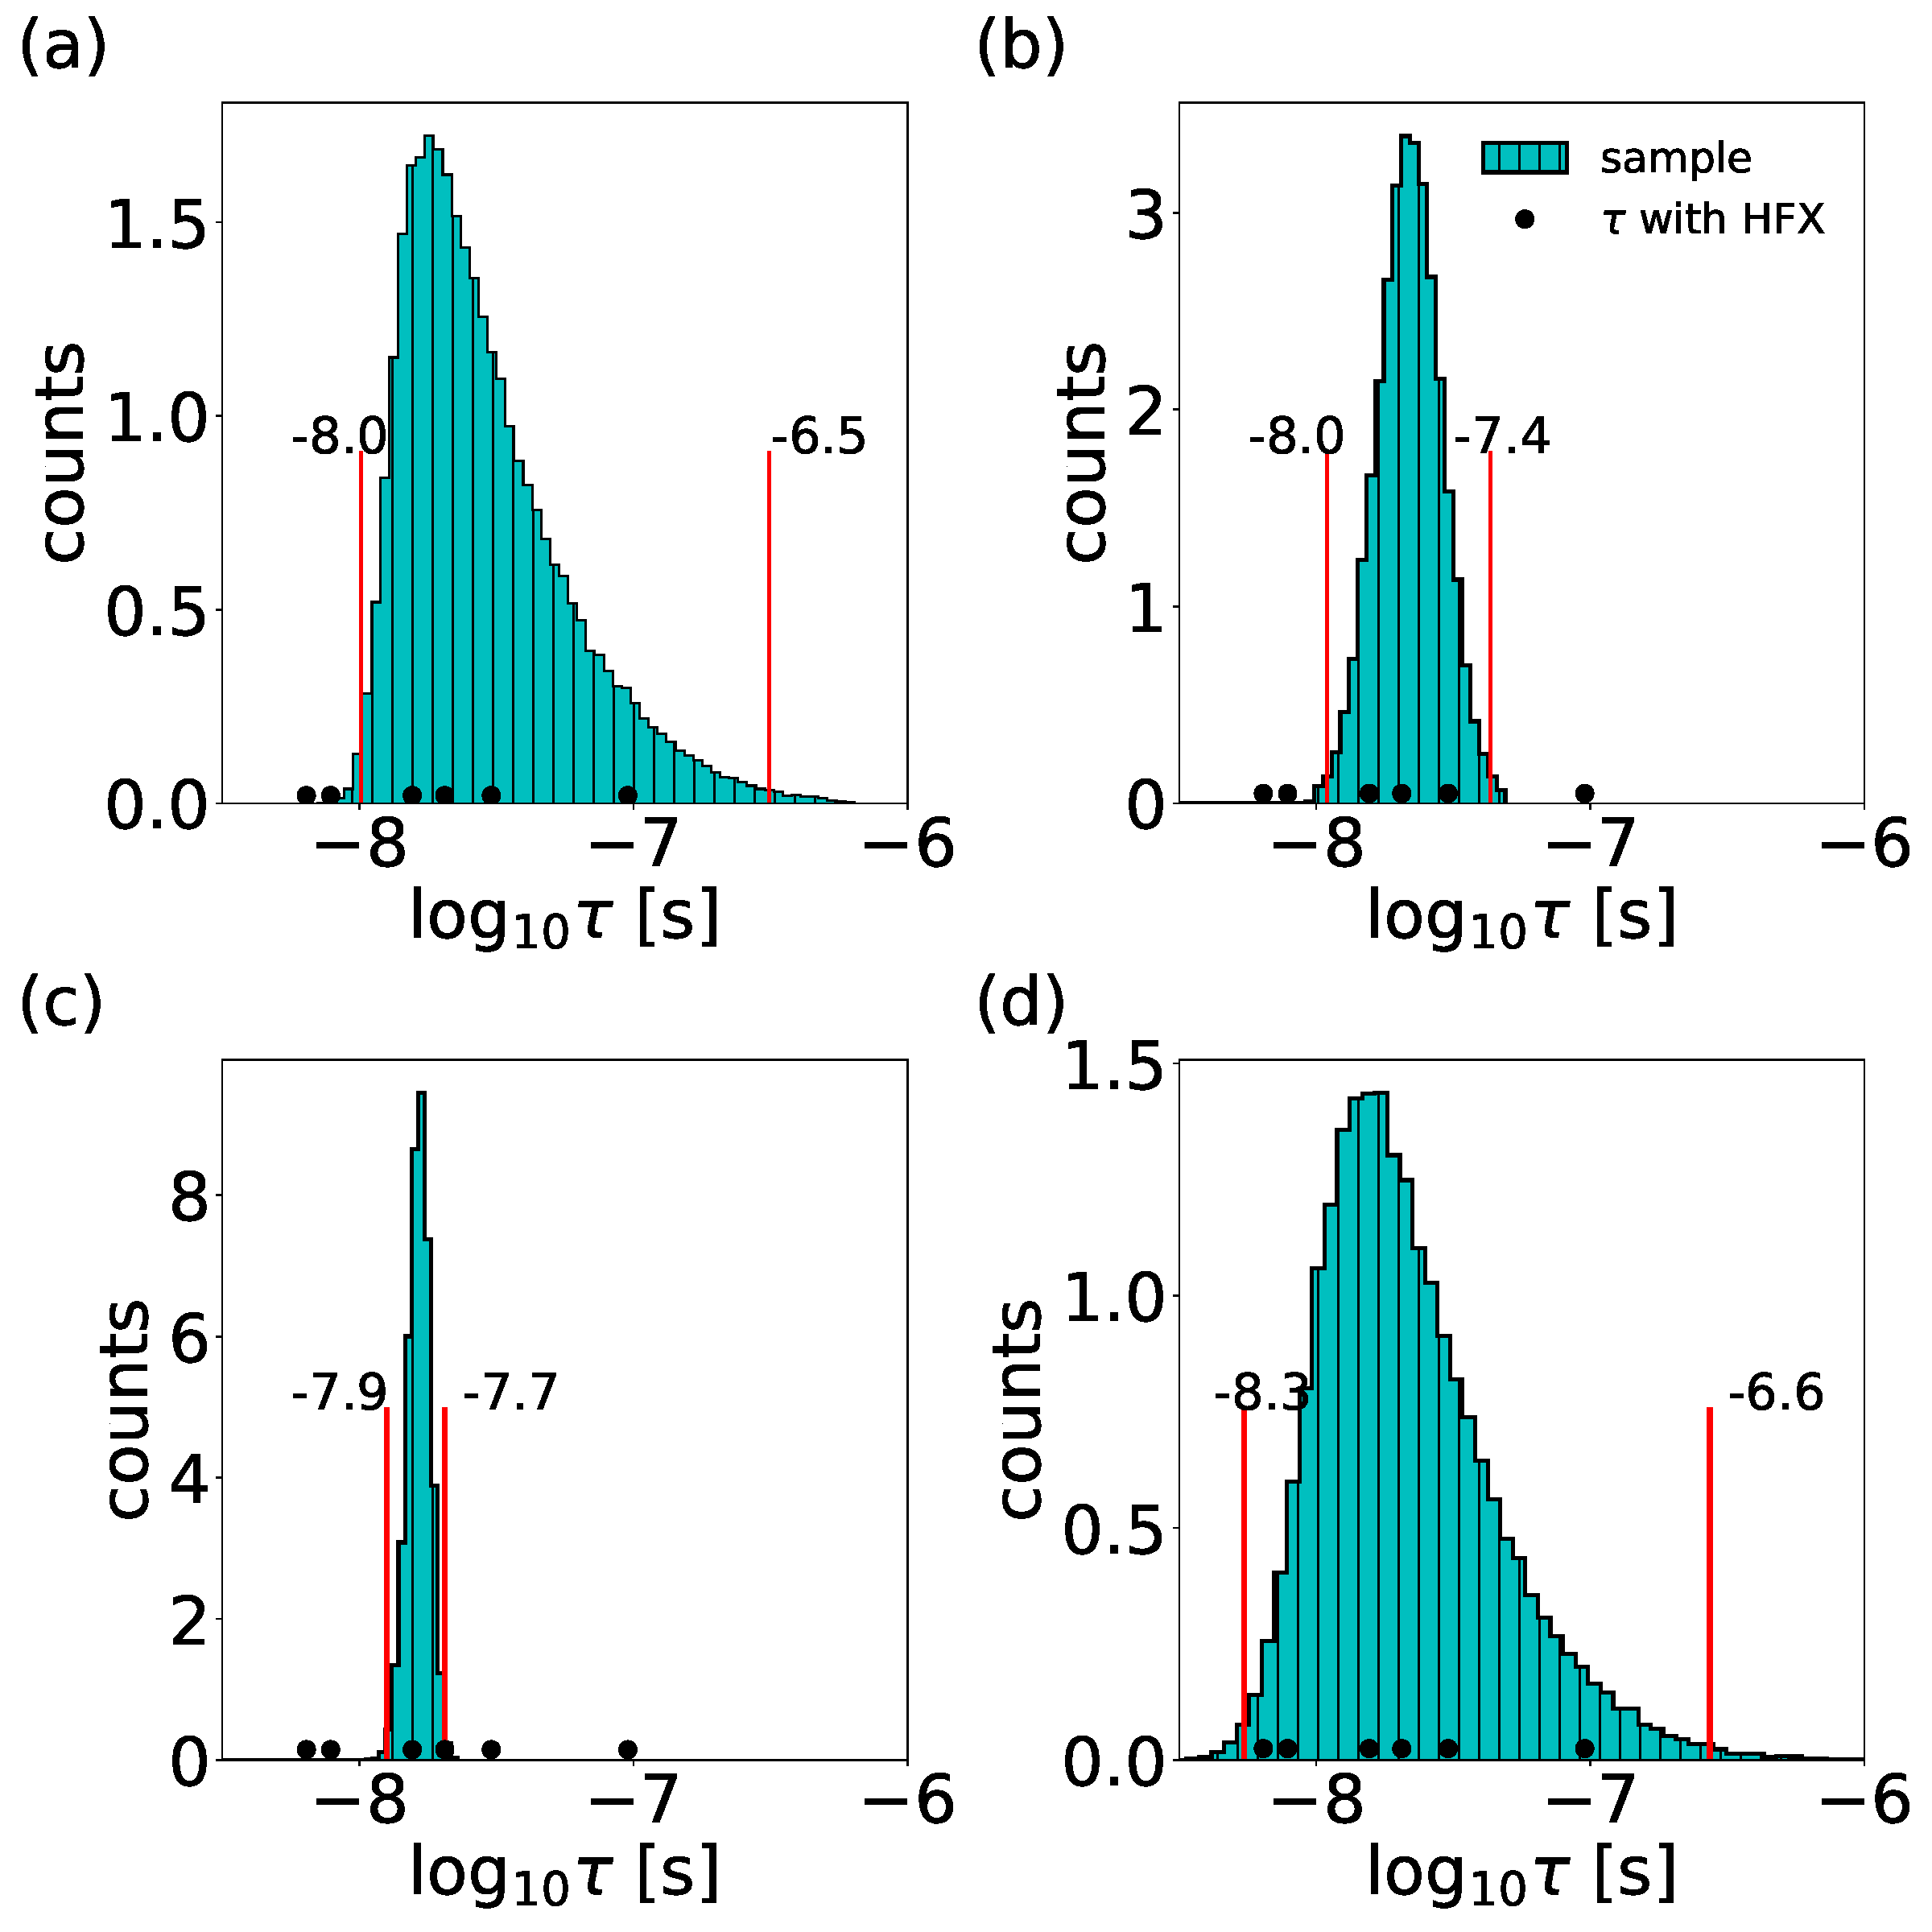
\includegraphics[width=0.45\textwidth]{figs/fig_mle_MADN_withE.pdf}
  \caption{\bjoern{TODO Zhong:}{these should also strictly be $\log_{10}(\tau/\unit[]{s})$.}Distribution of ToFs in the multiscale modeled MADN system.
  Monte Carlo sampling with a sample size $N_\text{MC}=50000$ is used to obtain the sampled distribution. The red vertical lines indicate the lower bound and upper bound of the 99\% confidence interval around the median.
  The black circles indicate the ToF obtained using varying HFX values.
  (a) $P(\log_{10}(\tau)|E_i \text{ uncertain})$, 
  (b) $P(\log_{10}(\tau)|\lambda \text{ uncertain})$, 
  (c) $P(\log_{10}(\tau)|J_{ij} \text{ uncertain})$, 
  (d) $P(\log_{10}(\tau)|E_i, \lambda, J_{ij} \text{ uncertain})$. }
  \label{fig:mle_MADN_withE}
\end{figure}
%


The distribution that we want to obtained during the parameter control are as followed:
\begin{enumerate}
    \item Fixed the $\lambda$ to be $\mathbb{E}(\lambda)$, and $\log_{10}(J_{ij}^2)$ to be $\mathbb{E}(\log_{10}(J_{ij}^2))$. Then each molecule energy $E_i$ is sampled from the normal distribution $\mathcal{N}(\mathbb{E}(E_i), \mathbb{V}(E_i))$. Finally obtain and plot the histogram $N_\text{MC}$ sample of $\tau$, whose distribution is denoted as $P(\log_{10}(\tau)|E_i \text{ uncertain})$.
    \item Fixed all $E_i$ to be $\mathbb{E}(E_i)$ and all $\log_{10}(J_{ij}^2)$ to be $\mathbb{E}(\log_{10}(J_{ij}^2))$. Then $\lambda$ is sampled from the normal distribution $\mathcal{N}(\mathbb{E}(\lambda), \mathbb{V}(\lambda))$. Finally obtain and plot the histogram  $N_\text{MC}$ sample of $\tau$, whose distribution is denoted as $P(\log_{10}(\tau)|\lambda \text{ uncertain})$. 
    \item Fixed the $\lambda$ to be $\mathbb{E}(\lambda)$ and all $E_i$ to be $\mathbb{E}(E_i)$.     Then $J_{ij}$ is sampled from the normal distribution $\log_{10}(J_{ij}^2) \in \mathcal{N}(\mathbb{E}(\log_{10}(J_{ij}^2)), \mathbb{V}(\log_{10}(J_{ij}^2)))$. Finally obtain and plot the histogram  $N_\text{MC}$ sample of $\tau$, whose distribution is denoted as $P(\log_{10}(\tau)|J_{ij} \text{ uncertain})$.
    \item Both $E_i$, $\lambda$ and $J_{ij}$ are sampled from their normal distribution:
    
    $\lambda_i \in \mathcal{N}(\mathbb{E}(\lambda), \mathbb{V}(\lambda))$, 
    
    $E_i \in \mathcal{N}(\mathbb{E}(E), \mathbb{V}(E))$, 
    
    $\log_{10}J_{ij}^2 \in \mathcal{N}(\mathbb{E}(\log_{10}J_{ij}^2), \mathbb{V}(\log_{10}J_{ij}^2))$.
    Then obtain and plot the histogram $N_\text{MC}$ sample of $\tau$, whose distribution is denoted as the following distribution: 
    $P(\log_{10}(\tau)|E_i, \lambda, J_{ij} \text{ uncertain})$.
\end{enumerate}

The ToF distribution for the MADN systems with energy disorder is shown in Fig.\ref{fig:mle_MADN_withE}.
The lower and upper bounds in Fig. \ref{fig:mle_MADN_withE} shows that when only the energies $E_i$ are uncertain, the $\log_{10}(\tau)$ has lower -8.0 and upper bound -6.5. This lower and upper bound is close to that of $P(\log_{10}(\tau)|E_i, \lambda, J_{ij} \text{ uncertain})$, meaning that varying the energy alone generates a $\tau$ distribution close to that when $E_i, \lambda, J_{ij}$ are uncertain. 

Figure .\ref{fig:mle_MADN_withE}(b) shows that $\log_{10}(\tau)$ has a confidence interval of -8.0 to -7.4 when $\lambda$ is varied. 
Figure \ref{fig:mle_MADN_withE}(c) show that when $J_{ij}$ is uncertain $\log_{10}(\tau)$ has a narrow confidence interval of -7.9 to -7.7, suggesting that the variation in $J_{ij}$ leads to relatively small change in $\log_{10}(\tau)$ compared to $E_i$ and $\lambda$.

%
\begin{figure}[t]
  \centering
  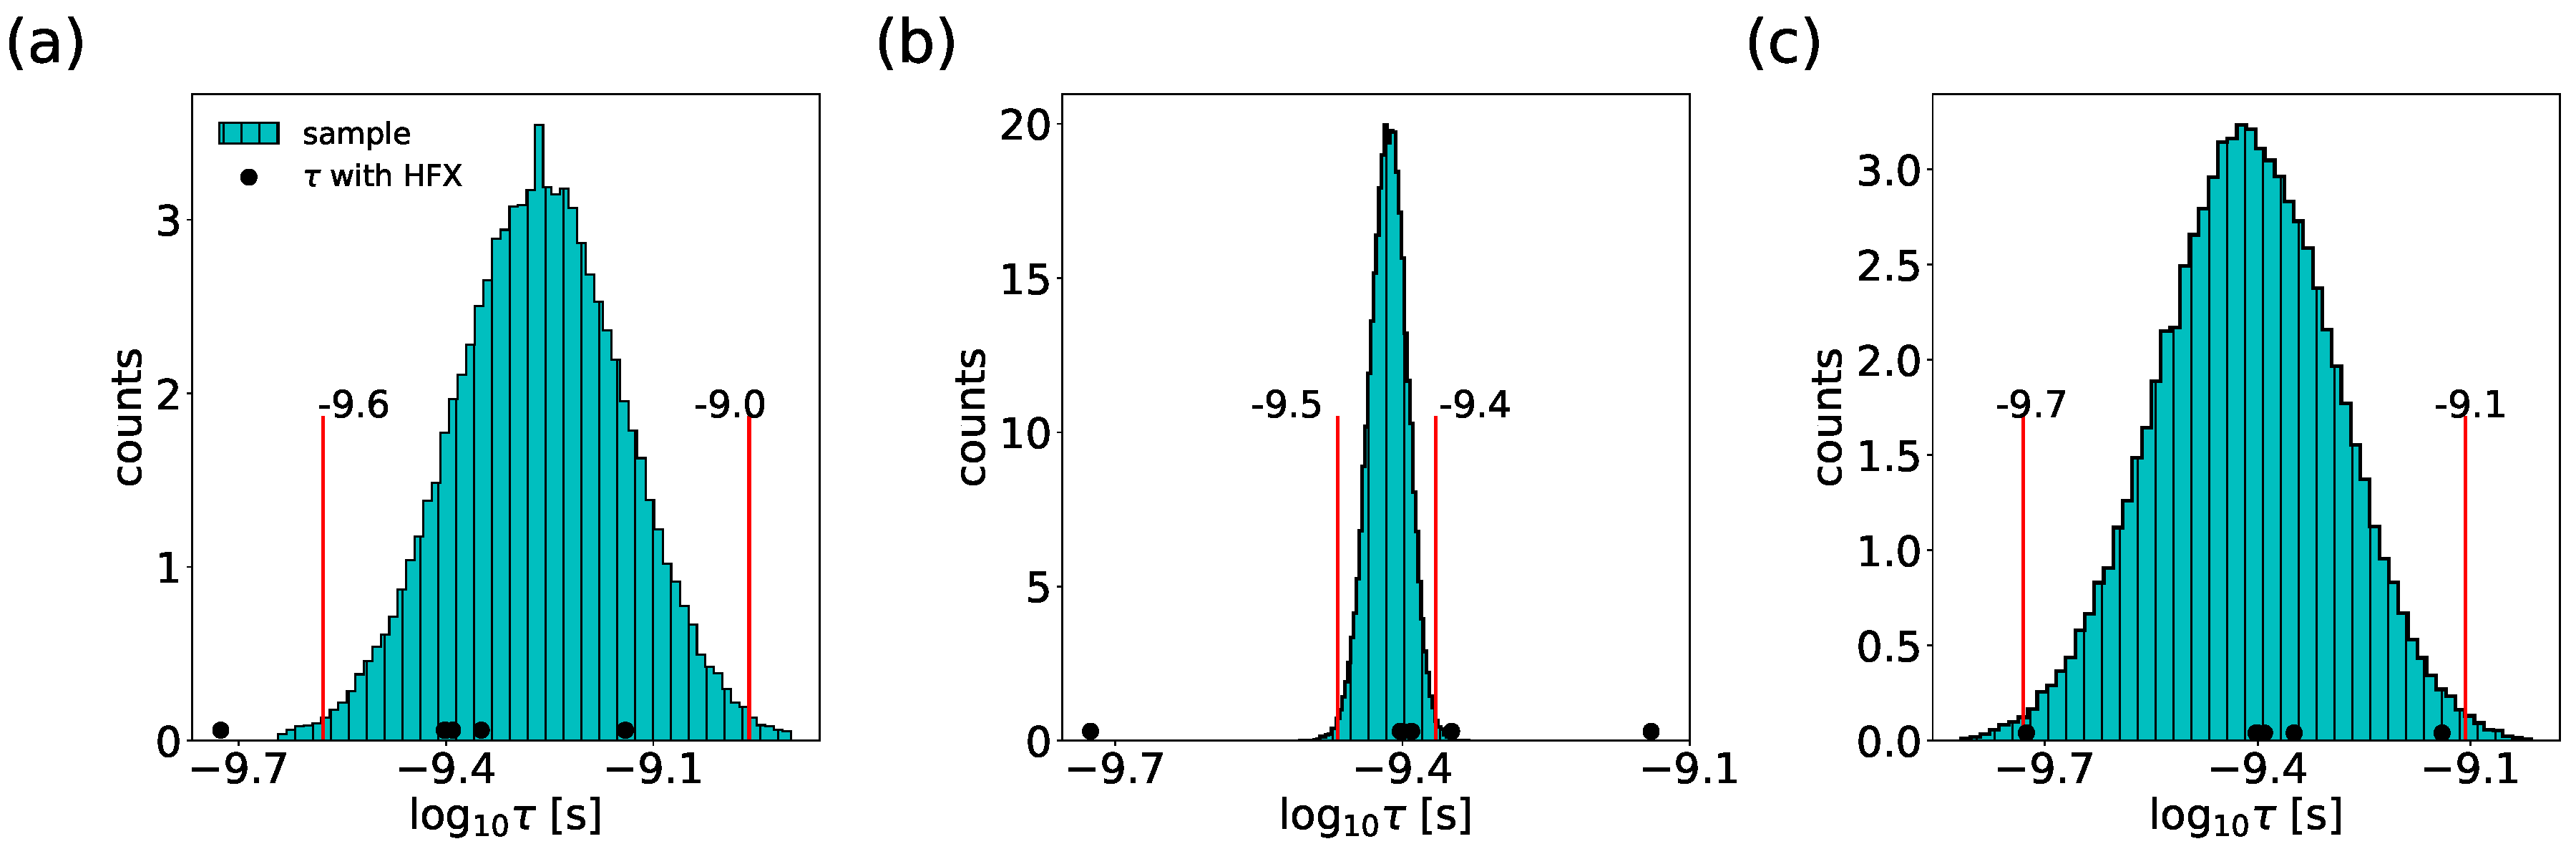
\includegraphics[width=0.45\textwidth]{figs/fig_mle_MADN_noE.pdf}
  \caption{\bjoern{TODO Zhong:}{these should also strictly be $\log_{10}(\tau/\unit[]{s})$.}Distribution of ToFs in the multiscale modeled MADN system.
  Monte Carlo sampling with a sample size $N_\text{MC}=50000$ is used to obtain the sampled distribution. The red vertical lines indicate the lower bound and upper bound of the 99\% confidence interval around the median.
  Energy disorder is not consider. 
  The black circles indicate the ToF obtained using varying HFX values.
  (a) $P(\log_{10}(\tau)|\lambda \text{ uncertain})$, 
  (b) $P(\log_{10}(\tau)|J_{ij} \text{ uncertain})$, 
  (c) $P(\log_{10}(\tau)|\lambda, J_{ij} \text{ uncertain})$. }
  \label{fig:mle_MADN_noE}
\end{figure}
%

When the energy disorder in MADN system is not considered, that is, all the MADN molecule energy are set to be equal giving $\Delta E=0$, the distribution of ToF is shown in Fig.\ref{fig:mle_MADN_noE}. 
The distribution $P(\log_{10}(\tau)|\lambda \text{ uncertain})$ has a range of confidence interval -9.6 to -9.0 resembles that of $P(\log_{10}(\tau)|\lambda, J_{ij} \text{ uncertain})$, which has a range of confidence interval -9.7 to -9.1. 

Measuring the sensitivity of each electronic parameter to ToF is to measure each electronic parameter's contribution to the variance of ToF. 
That is, if ToF is most sensitive to one parameter, the variance in this particular parameter will contribute most to the ToF variance. 


One way of decomposing the variance of the model output into fractions attributed to input parameters is the variance-based sensitivity analysis. The local sensitive analysis is to use the partial derivative $\frac{\partial \tau}{\partial x_i}$. While the global sensitivity analysis can use Sobol's indices. Given a model of Equation \ref{eq:tau1}, to measure the parameter $x_i$'s contribution to $\tau$ including all variance caused by its interaction with other parameters $\{x_k, k \neq i \}$, the total effect Sobol's index is calculated as \cite{saltelli_variance_2010}:
\begin{equation}
    S_{T,i} = \frac{ \mathbb{E}_{\mathbf{x}_{\sim i}}[ \mathbb{V}_{x_i}(\tau|\mathbf{x}_{\sim i}) ] }{ \mathbb{V}(\tau) }
    \label{eq:STi}
\end{equation}
The details of the notation is as followed: the vector $\mathbf{x}=(x_1, x_2, \cdots, x_{N_d})$, and $\mathbf{x}_{\sim i}$ denotes the vector of all entries but $x_i$. 
$\mathbb{V}_{x_i}(\tau|\mathbf{x}_{\sim i})$ means the variance of $\tau$ given a set of $\mathbf{x}_{\sim i}$ taken over $x_i$. And $ \mathbb{E}_{\mathbf{x}_{\sim i}}[\cdot]$ denotes the mean of argument $(\cdot)$ taken over all factors but $x_i$.

%
\begin{table}[tbp]%The best place to locate the table environment is directly after its first reference in text
\caption{\label{tab:Sobol}%
Sobol indices of $\lambda$, $E$ and $\log_{10} J^2$ when ToF is calculated with energy disorder, and Sobol indices of $\lambda$ and $\log_{10} J^2$ when ToF is calculated without energy disorder.
}
\begin{ruledtabular}
  \begin{center}
    \begin{tabular}{c c c c c c c} %\hline
      &  \multicolumn{3}{c}{\bf Energy Disorder} & &\multicolumn{2}{c}{\bf no Disorder}\\\cline{2-4}  \cline{6-7}
      parameter  & $\lambda$ & $ E_i$ & $ \log_{10}(J_{ij}^2)$ && $\lambda$ & $ \log_{10}(J_{ij}^2)$ \\ \hline
      %\multicolumn{6}{c}{\bf GRW for $\mathbf{N_c=1}$}\\
   $S_T$  & 0.097 & 0.95 & 0.018 && 0.96 & 0.11 \\
    \end{tabular}
  \end{center}
\end{ruledtabular}
\end{table}
%
Then the $\lambda$ contribution to the total variance is $S_{T,i=1}$.
The energy contribution to the total variance is $S_{T,E} = \sum\limits_{i=1}^{N+1} S_{T,i}$ where $N=1000$ is the number of energy parameter, and the coupling element contribution due to variation in $\log_{10}(J_{ij}^2)$ to the total variance is $S_{T,J}=\sum\limits_{i=N+2}^{N_d} S_{T,i}$. 
Using the quasi Monte Carlo method\cite{sobol_global_2001} with a sample size $N_\text{QMC}=1000$ to calculate $S_{T,i}$, the results are shown in the table \ref{tab:Sobol}.

From table \ref{tab:Sobol} one can see that most of the total variance can be attributed to the energy $E$. In contrast to $E$, the uncertainty in $\lambda$ and $\log_{10} J^2$ contributes much less compared to $E$, this is consistent to the Fig.\ref{fig:mle_MADN_withE}, where the distribution in Fig.\ref{fig:mle_MADN_withE}(d) resembles the distribution in Fig.\ref{fig:mle_MADN_withE}(a).
And Fig.\ref{fig:mle_MADN_withE}(c) shows that the uncertainty in $\log_{10}(J^2)$ only leads to small variances.
When there is no energy disorder, the variance in $\lambda$ has the most contribution to the total variance as shown in Table \ref{tab:Sobol}.

%%%%%%%%%%%%%%%%%%%%%%%%%%%%%%%%%%%%%%%%%%%%%%%%%%%%%%%%%%%%%%%%%%%
%
%\begin{figure}
%  \centering
%  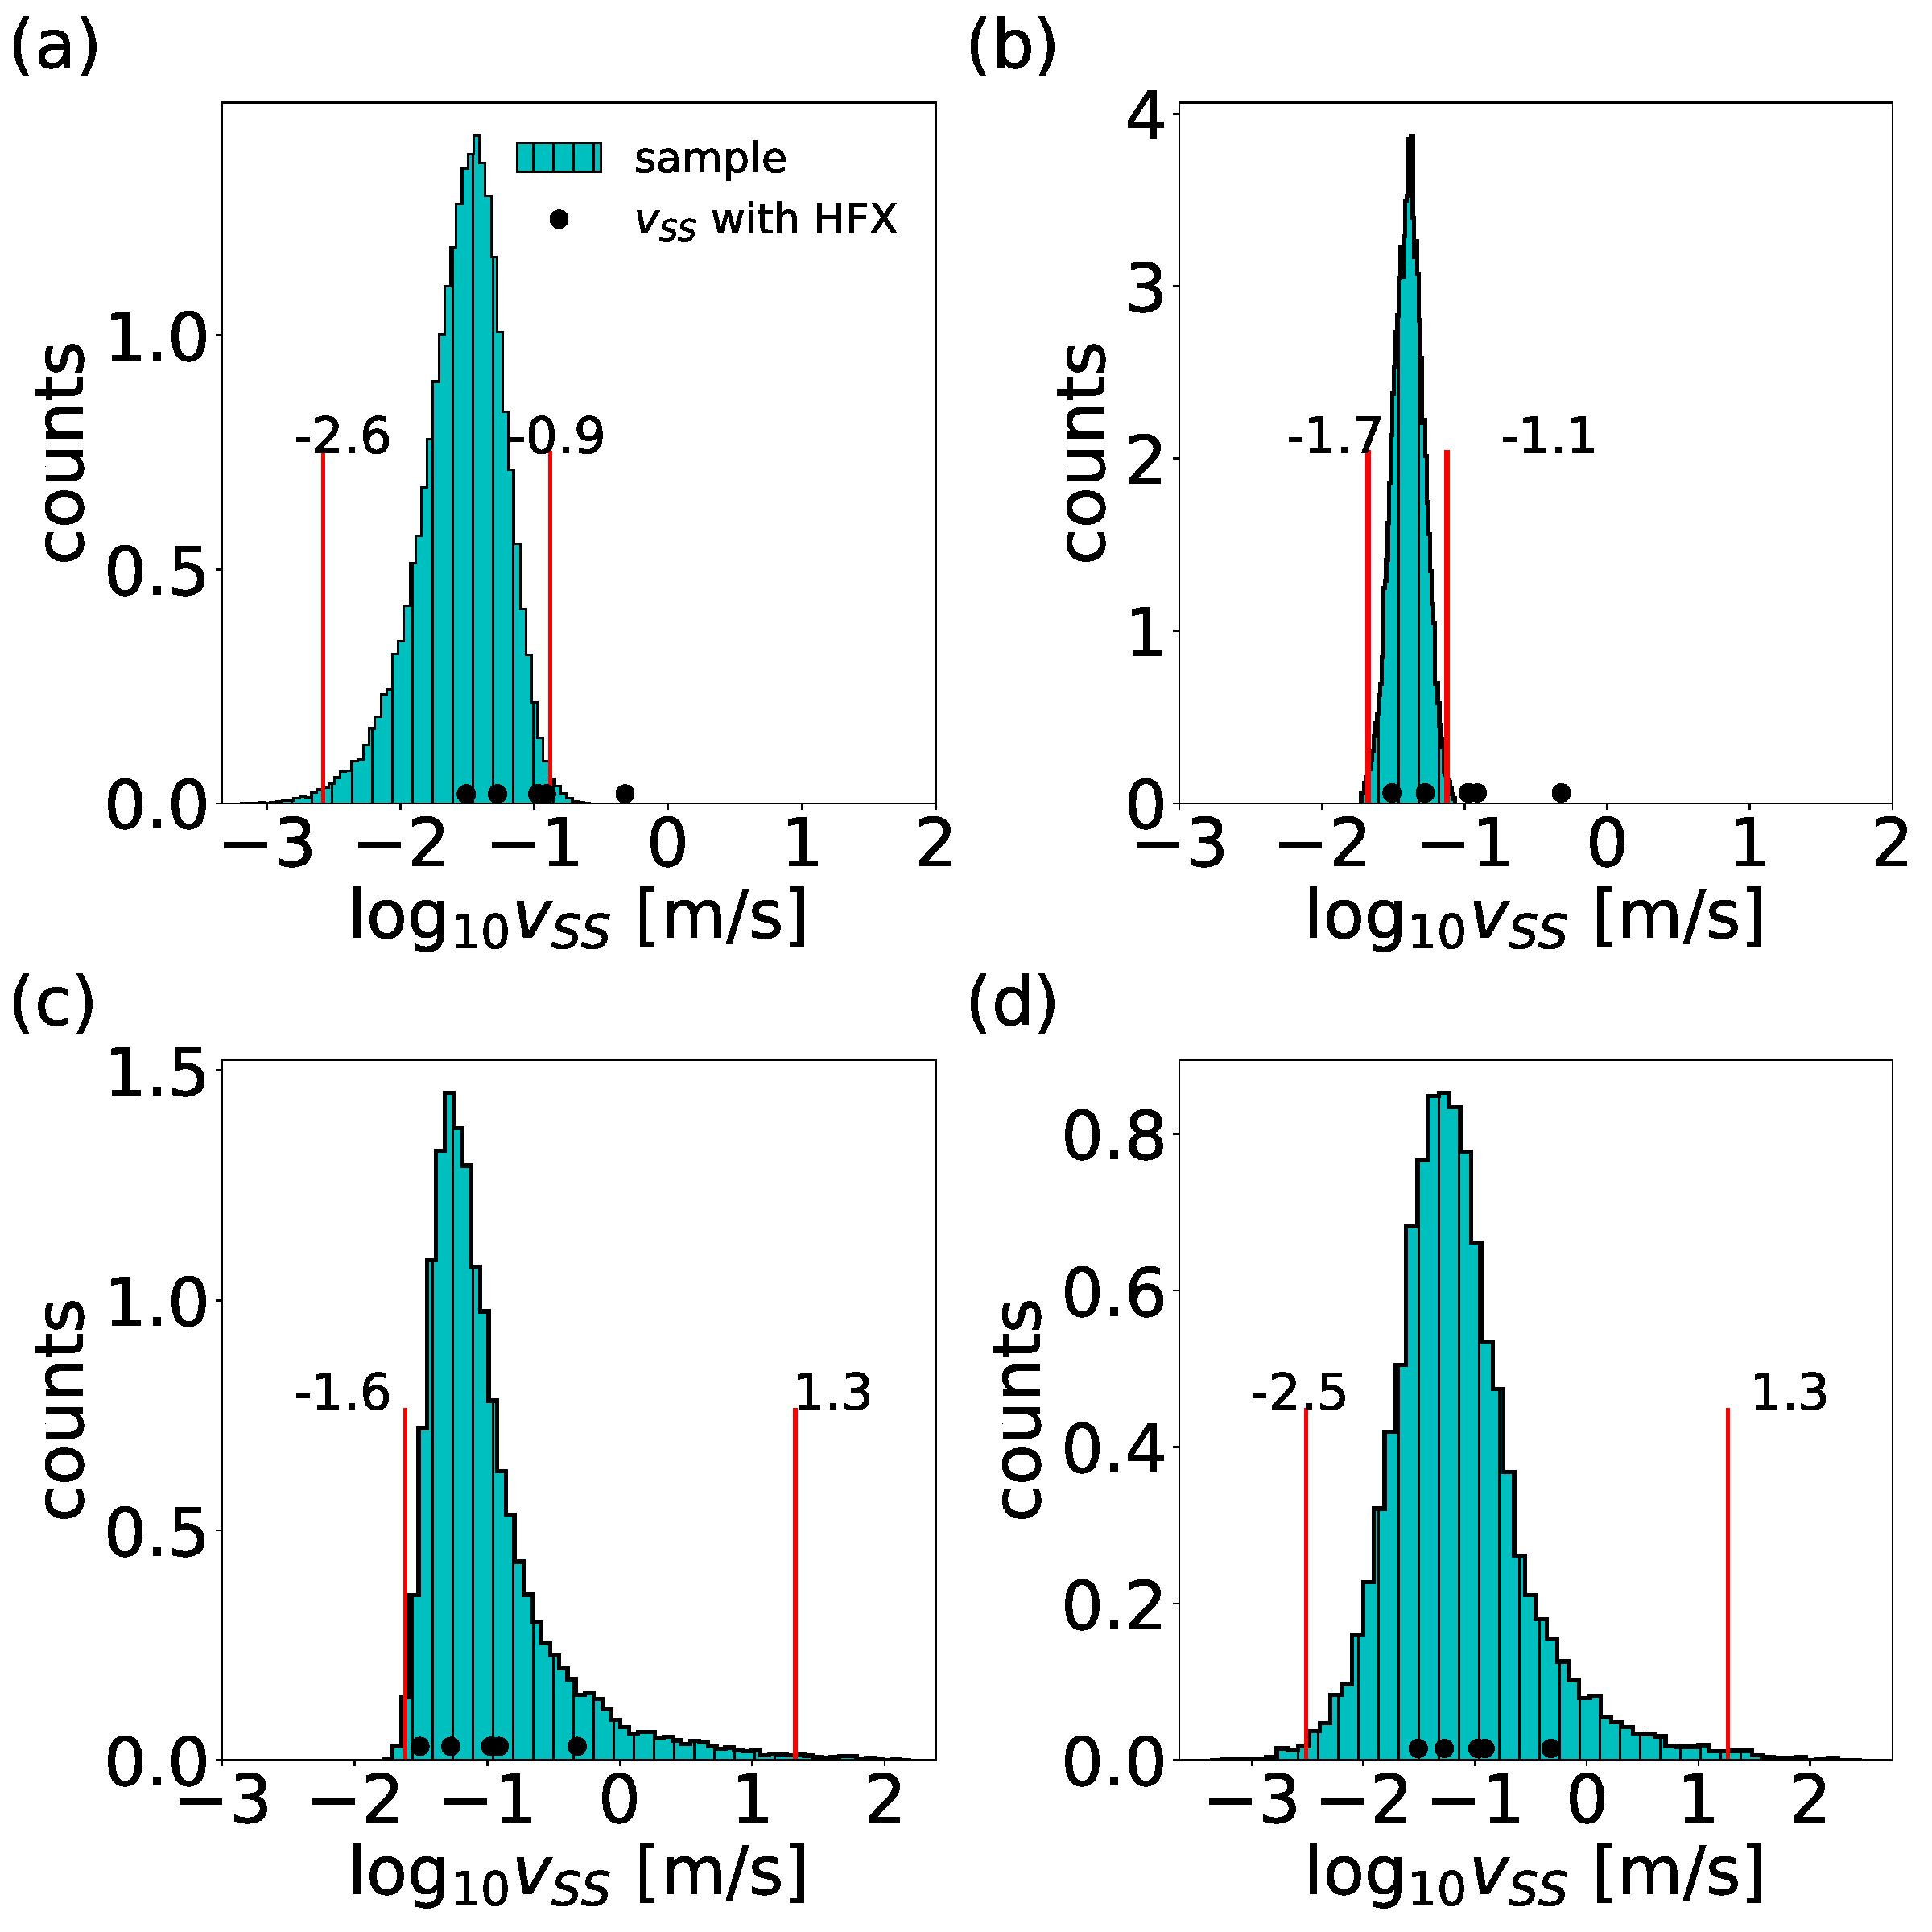
\includegraphics[width=0.45\textwidth]{figs/fig_mle_MADN_withE_SS.pdf}
%  \caption{Distribution of steady state velocity $v_\text{SS}$ in the multiscale modeled MADN.
%  Monte Carlo sampling with a sample size $N_\text{MC}=50000$ is used to obtain the sampled distribution.
%  The red vertical lines indicate the lower bound and upper bound of the 99\% confidence interval around the median.
%  The black circles indicate the $v_\text{SS}$ obtained using varying HFX values.
%  (a) $P(\log_{10}(v_\text{SS})|E_i \text{ uncertain})$, 
%  (b) $P(\log_{10}(v_\text{SS})|\lambda \text{ uncertain})$, 
%  (c) $P(\log_{10}(v_\text{SS})|J_{ij} \text{ uncertain})$, 
%  (d) $P(\log_{10}(v_\text{SS})|E_i, \lambda, J_{ij} \text{ uncertain})$. }
%  \label{fig:mle_MADN_withE_SS}
%\end{figure}
%
%
%\begin{figure}
%  \centering
%  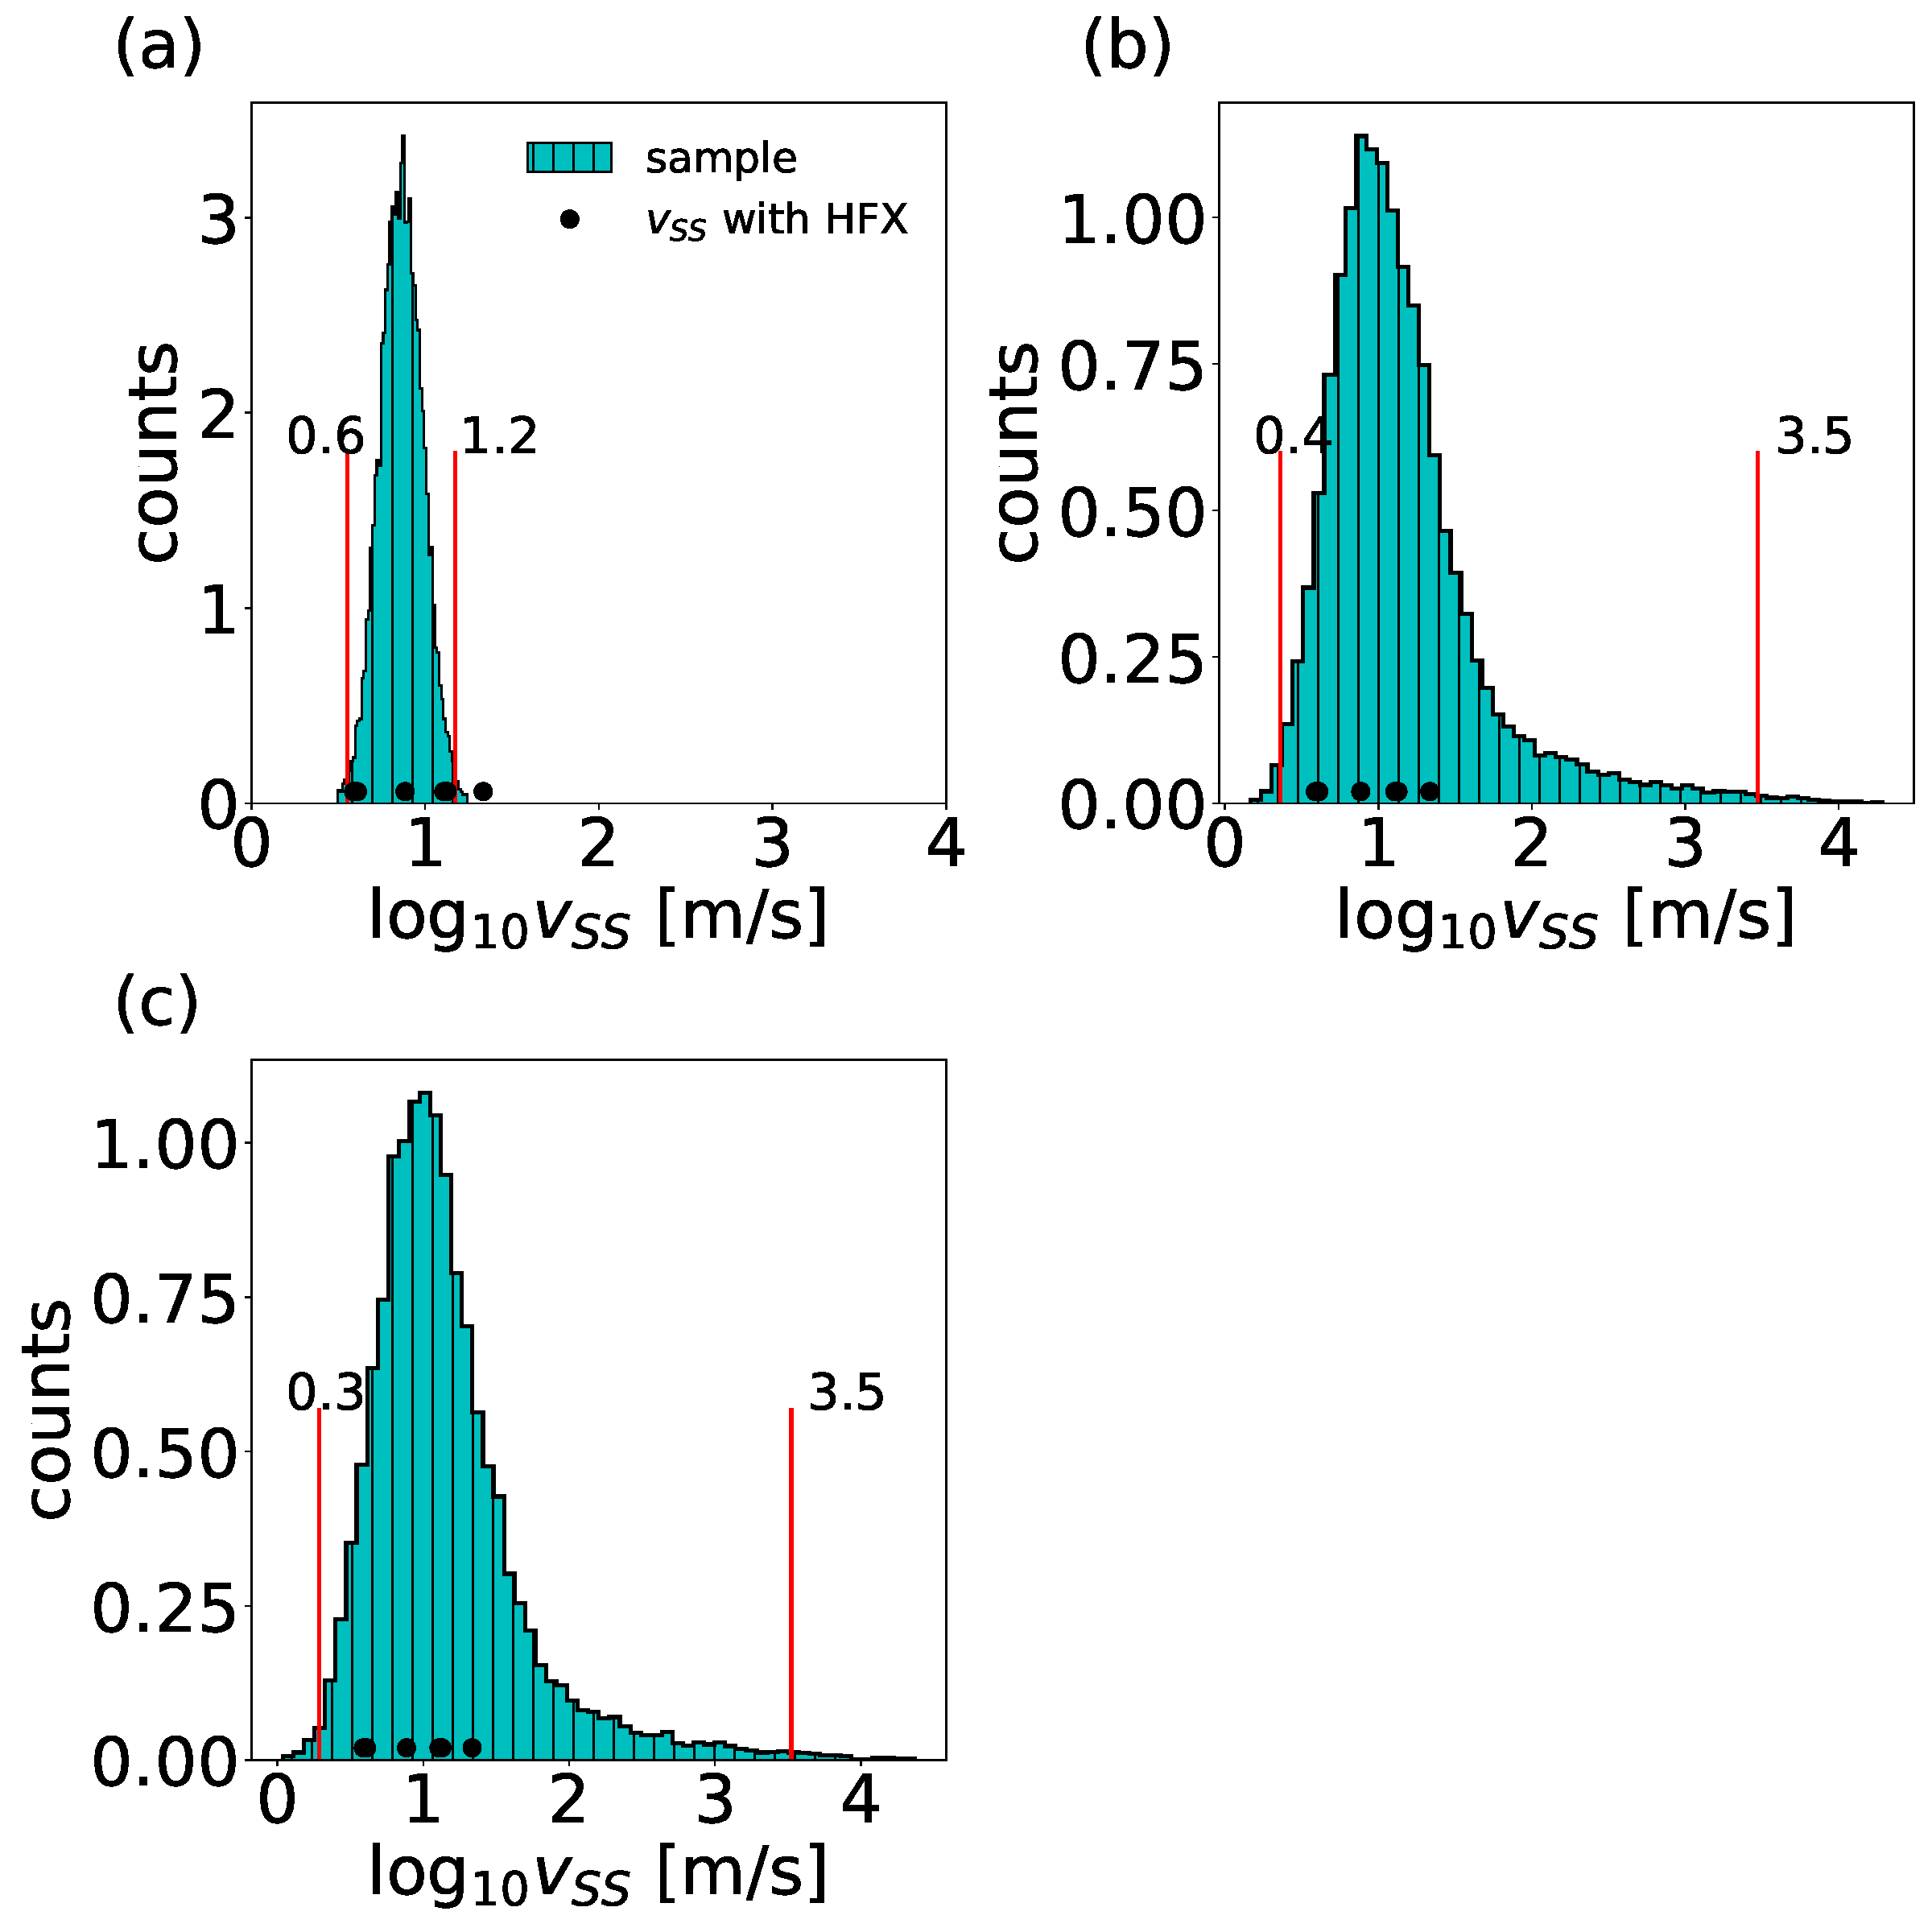
\includegraphics[width=0.45\textwidth]{figs/fig_mle_MADN_noE_SS.pdf}
%  \caption{Distribution of steady state velocity $v_\text{SS}$ in the multiscale modeled MADN. All molecule energies are set to be zero.  
%  Monte Carlo sampling with a sample size $N_\text{MC}=50000$ is used to obtain the sampled distribution.
%  The red vertical lines indicate the lower bound and upper bound of the 99\% confidence interval around the median.
%  The black circles indicate the $v_\text{SS}$ obtained using varying HFX values.
%  (a) $P(\log_{10}(v_\text{SS})|\lambda \text{ uncertain})$, 
%  (b) $P(\log_{10}(v_\text{SS})|J_{ij} \text{ uncertain})$, 
%  (c) $P(\log_{10}(v_\text{SS})|\lambda, J_{ij} \text{ uncertain})$.  }
%  \label{fig:mle_MADN_noE_SS}
%\end{figure}


%\section{Distribution of Steady State Velocity}

%The distribution of steady state velocity of MADN is shown as Fig.\ref{fig:mle_MADN_withE_SS} and \ref{fig:mle_MADN_noE_SS}. 
%From the confidence interval, $P(\log_{10}(v_\text{SS})|E_i \text{ uncertain})$ has a range of -2.6 to -0.9, and the confidence interval $P(\log_{10}(v_\text{SS})|\lambda \text{ uncertain})$ has a range from -1.7 to -1.1. The width of those confidence intervals is very close to the confidence interval of distributions $P(\log_{10}(\tau)|E_i \text{ uncertain})$ and $P(\log_{10}(\tau)|\lambda \text{ uncertain})$, respectively.
%However, $P(\log_{10}(v_\text{SS})|J_{ij} \text{ uncertain})$ has a range from -1.6 to 1.3, spanning 3 orders of magnitude. This is  much larger than $P(\log_{10}(\tau)|J_{ij} \text{ uncertain})$ as shown in Fig .\ref{fig:mle_MADN_withE}.  
%The large confidence interval in $P(\log_{10}(v_\text{SS})|J_{ij} \text{ uncertain})$ shows that $v_{ss}$ is very sensitive to the change in $J_{ij}$. Combining all the uncertainty effects in $E_i, \lambda, J_{ij}$, the confidence interval of $P(\log_{10}(v_\text{SS})|E_i, \lambda, J_{ij} \text{ uncertain})$ is from -2.5 to 1.3, covering 4 orders of magnitude.  

%When energy disorder is not considered, the $v_\text{SS}$ distribution $P(\log_{10}(v_\text{SS})|\lambda, J_{ij} \text{ uncertain})$ has a confidence interval from 0.3 to 3.5, spanning 3 orders of magnitude. This interval is close to the range of $P(\log_{10}(v_\text{SS})|J_{ij} \text{ uncertain})$ when only $J_{ij}$ is uncertain. 
%In contrast, the interval of $P(\log_{10}(v_\text{SS})|\lambda \text{ uncertain})$ is from 0.6 to 1.2, whose width is much smaller than that of $P(\log_{10}(v_\text{SS})|J_{ij} \text{ uncertain})$.

%These result suggests that compared to the ToF $\tau$, the quantity $v_\text{SS}$ is significantly affected by uncertainties in $J_{ij}$, so $v_\text{SS}$ is less robust when the parameters $E_i, \lambda, J_{ij}$ contains uncertainty at the same time. 
%In the next section, the Poole–Frenkel behavior, that is the dependence of charge mobility on the electric field will be study using the ToF setting. 
%%%%%%%%%%%%%%%%%%%%%%%%%%%%%%%%%%%%%%%%%%%%%%%%%%%%%%%%%%%%%%%%%%%%%%%%%%

\section{Charge mobility and PF Behavior}

In this section, we want to study the dependence of drift mobility on the HFX. The charge mobility is calculated as:
\begin{equation}
    \mu = \frac{\vec{v} \vec{F} }{ |\vec{F}|^2}
    \label{eq:mu}
\end{equation}
To consider the charge dynamics along X, Y and Z axis in the ToF setting, the ToF is calculated with different settings of \textit{Source}-\textit{Sink} and $\vec{F}$ combinations.

\begin{itemize}
    \item Setting the molecules with $r^x < \min(r^x)+0.5$ as \textit{Source}, and the molecules with $r^x > \max(r^x)-0.5$ as \textit{Sink}, and $\vec{F}^T = (F,0,0)$, denote the calculated the ToF as $\tau_\text{Xmin}$, and the mobility is as $\mu_\text{Xmin} = \frac{L_x }{\tau_\text{Xmin} |\vec{F}|}$.  
    \item Setting the molecules with $r^x > \max(r^x)-0.5$ as \textit{Source}, and the molecules with $r^x < \min(r^x)+0.5$ as \textit{Sink}, and $\vec{F}^T = (-F,0,0)$, denote the calculated the ToF as $\tau_\text{Xmax}$, and the mobility is as $\mu_\text{Xmax} = \frac{L_x }{\tau_\text{Xmax} |\vec{F}|}$.  
    \item Setting the molecules with $r^y < \min(r^y)+0.5$ as \textit{Source}, and the molecules with $r^y > \max(r^y)-0.5$ as \textit{Sink}, and $\vec{F}^T = (0,F,0)$, denote the calculated the ToF as $\tau_\text{Ymin}$, and the mobility is as $\mu_\text{Ymin} = \frac{L_y }{\tau_\text{Ymin} |\vec{F}|}$. 
    \item Setting the molecules with $r^y > \max(r^y)-0.5$ as \textit{Source}, and the molecules with $r^y > \max(r^y)-0.5$ as \textit{Sink}, and $\vec{F}^T = (0,-F,0)$, denote the calculated the ToF as $\tau_\text{Ymax}$, and the mobility is as $\mu_\text{Ymax} = \frac{L_y }{\tau_\text{Ymax} |\vec{F}|}$. 
    \item Setting the molecules with $r^z < \min(r^z)+0.5$ as \textit{Source}, and the molecules with $r^z > \max(r^z)-0.5$ as \textit{Sink}, and $\vec{F}^T = (0,0,F)$, denote the calculated the ToF as $\tau_\text{Zmin}$, and the mobility is as $\mu_\text{Zmin} = \frac{L_z }{\tau_\text{Zmin} |\vec{F}|}$. 
    \item Setting the molecules with $r^z > \max(r^z)-0.5$ as \textit{Source}, and the molecules with $r^z > \min(r^z)+0.5$ as \textit{Sink}, and $\vec{F}^T = (0,0,-F)$, denote the calculated the ToF as $\tau_\text{Zmax}$, and the mobility is as $\mu_\text{Zmax} = \frac{L_z }{\tau_\text{Zmax} |\vec{F}|}$. 
\end{itemize}
Finally the ToF drift mobility is calculated as:
\begin{equation}
    \mu_\text{PF} = \frac{1}{6} (\mu_\text{Xmin}+\mu_\text{Xmax}+\mu_\text{Ymin}+\mu_\text{Ymax}+\mu_\text{Zmin}+\mu_\text{Zmax})
\end{equation}

When the $\lambda, E_i, J_{ij}$ are uncertain and sampled from the normal distribution, the distributions of charge mobility obtained from MC sample under specific electric field are shown in Fig.\ref{fig:fig_mle_withE_mu2_ave}.
%
\begin{figure}
    \centering
    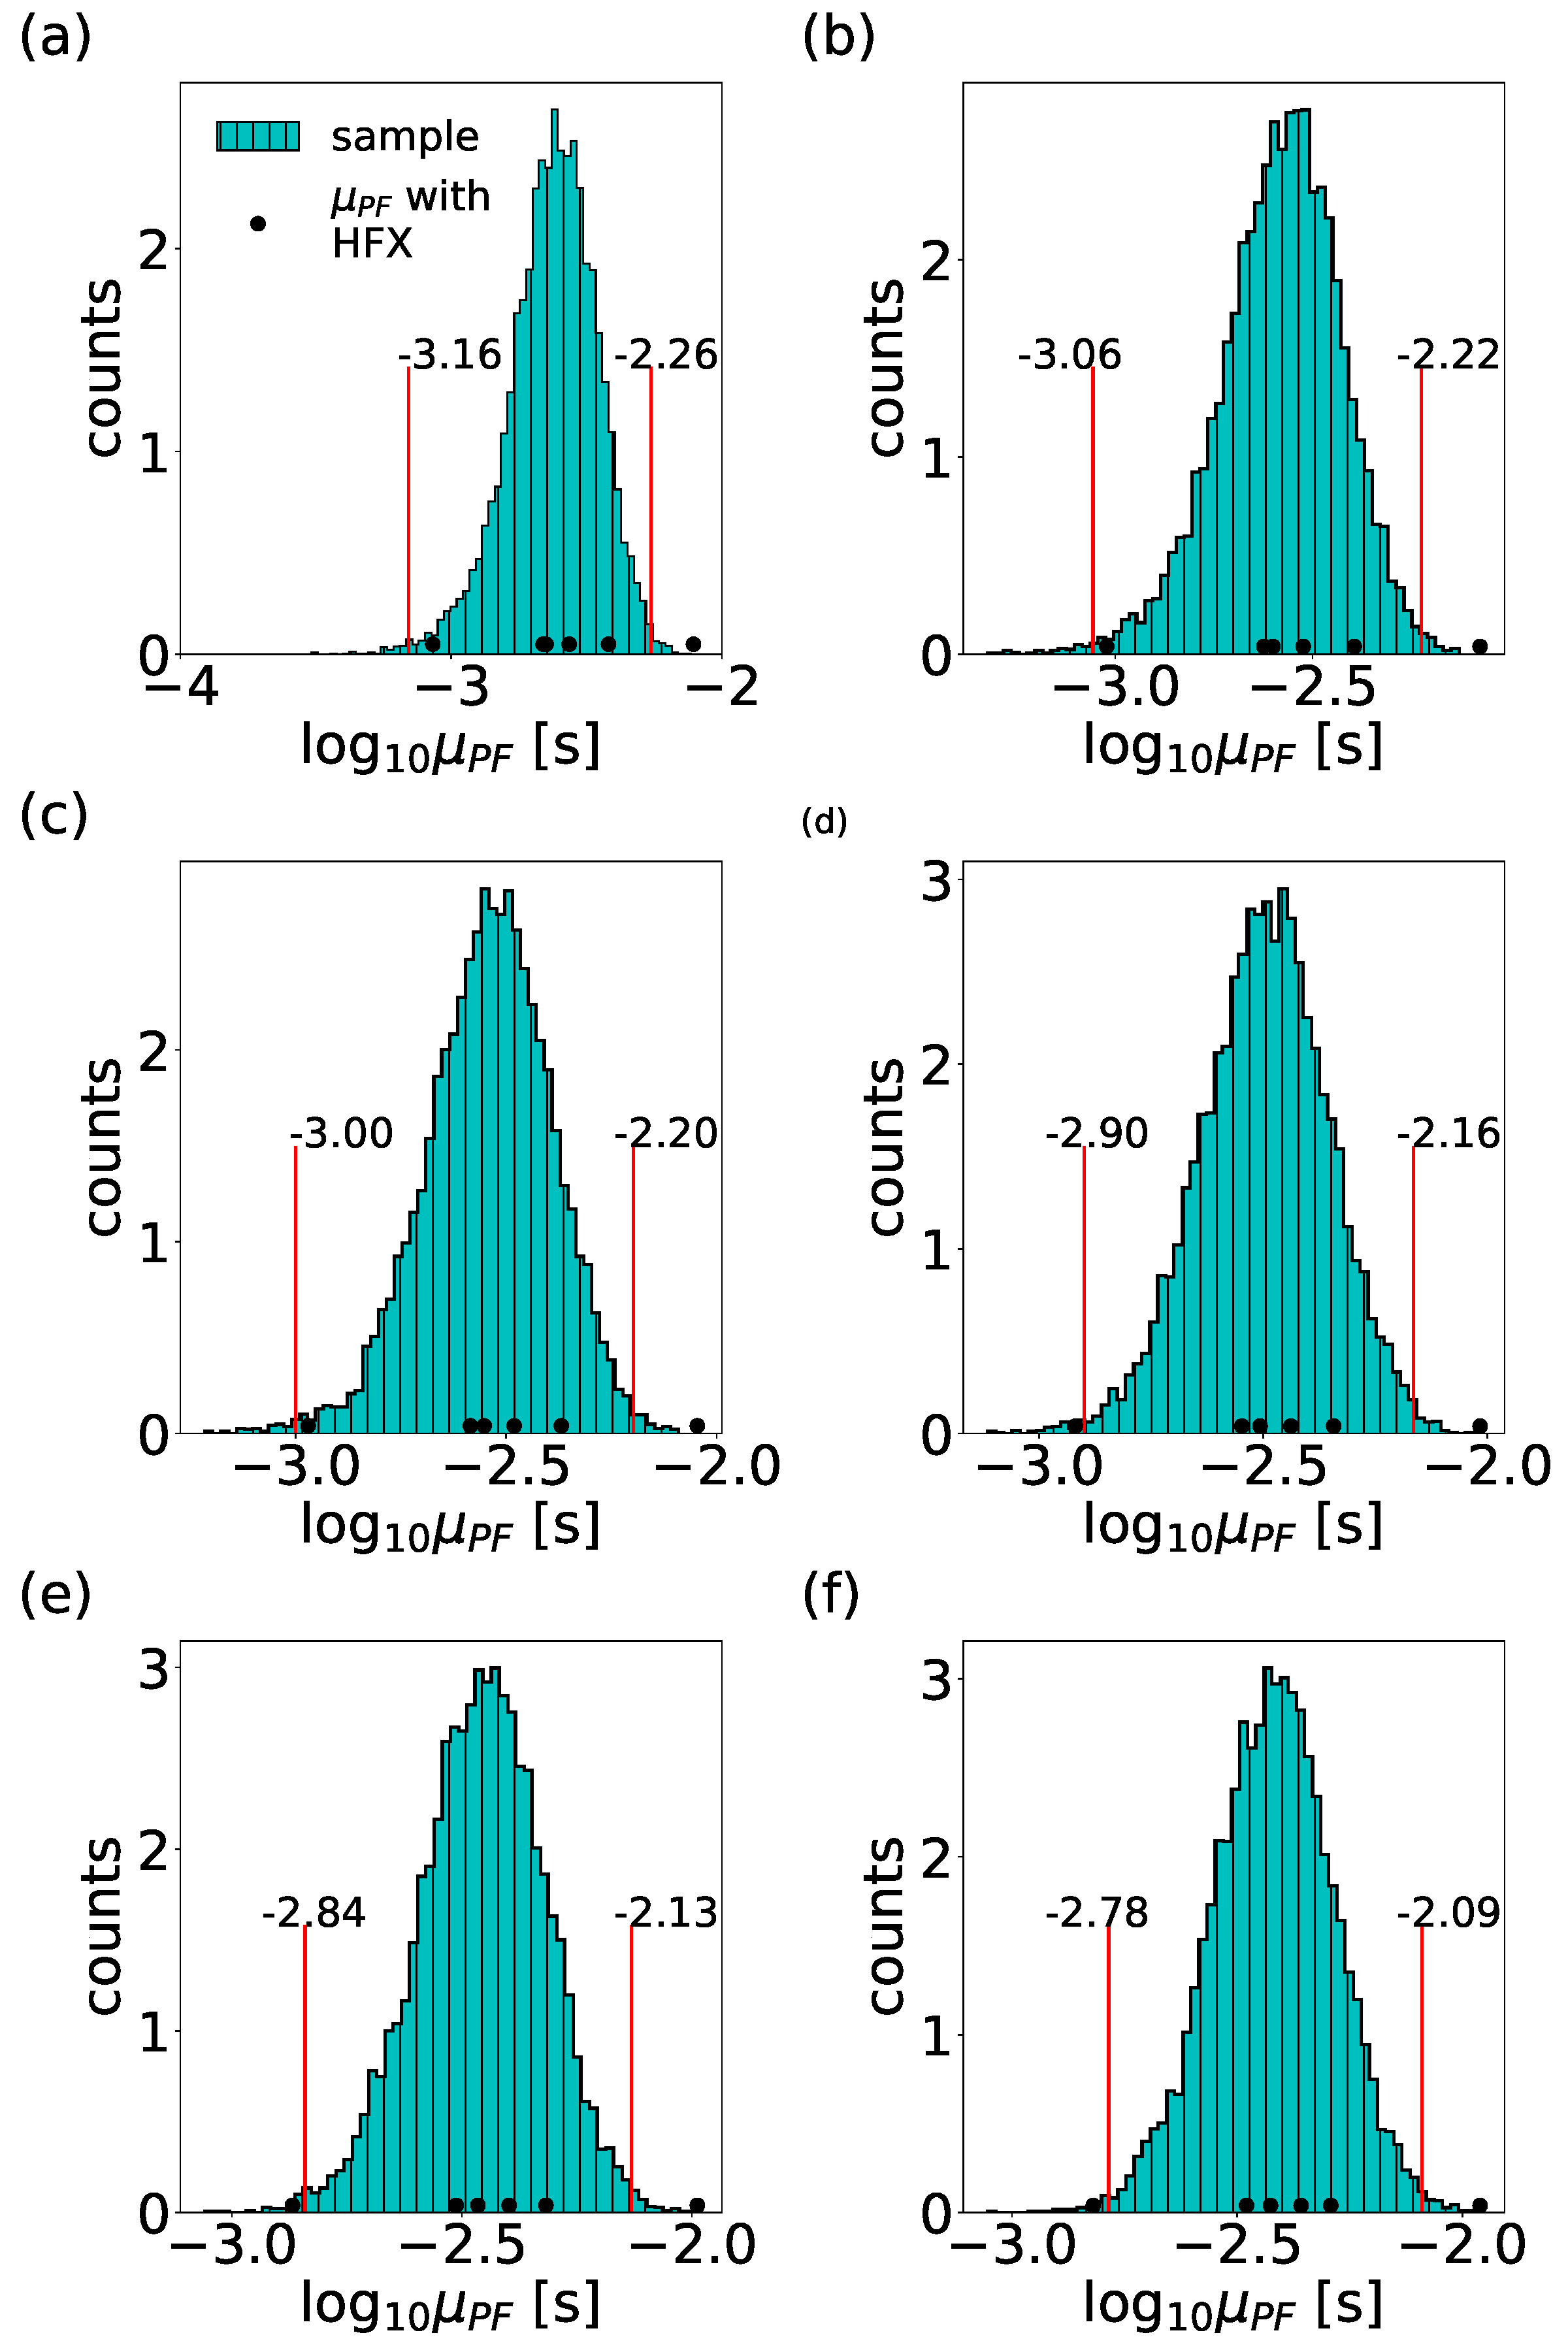
\includegraphics[width=0.45\textwidth]{figs/fig_mle_withE_mu2_ave.pdf}
    \caption{\bjoern{TODO Zhong:}{these should also strictly be $\log_{10}(\mu/(\unit[]{cm^2(Vs)^{-1}}))$; there should be no PF label at $\mu$.} Distribution of $\mu_\text{PF}$ in the multiscale modeled MADN system.
    Monte Carlo sampling with a sample size $N_\text{MC}=10000$ is used to obtain the sampled distribution. The red vertical lines indicate the lower bound and upper bound of the 99\% confidence interval around the median. (a) $|\vec{F}|=4 \times 10^7 \unit{V/m}$, (b) $|\vec{F}|=5 \times 10^7 \unit{V/m}$, (c) $|\vec{F}|=6 \times 10^7 \unit{V/m}$, (d) $|\vec{F}|=7 \times 10^7 \unit{V/m}$, (e) $|\vec{F}|=8 \times 10^7 \unit{V/m}$, (f) $|\vec{F}|=9 \times 10^7 \unit{V/m}$.}
    \label{fig:fig_mle_withE_mu2_ave}
\end{figure}
%

When the $\lambda, E_i, J_{ij}$ are uncertain and sampled from the normal distribution, the distributions of charge mobility obtained from MC sample under specific electric field are shown in Fig. \ref{fig:fig_mle_withE_mu2_ave}. The ToF depends on the electric field through the Marcus rate. As the electric increase from $|\vec{F}|=4 \times 10^7 \unit{V/m}$
$|\vec{F}|=9 \times 10^7 \unit{V/m}$, the
range of the 90\% confidence interval where $\log_{10} \mu_\text{PF}$ lies
estimated from the MC sample decrease from 0.90 to 0.69.
So the electric field results in a narrower range of $\mu_\text{PF}$ distribution.
Due to this reason, the $\mu_\text{PF}$ calculated from $\alpha=0$ is not in the 99\% confidence interval around the median of the MC sampled data, although the zero-field ToF of $\alpha=0$ is contained in the according 99\% confidence interval, as shown in Fig. \ref{fig:mle_MADN_withE}(d).

The ToF depends on the electric field through the Marcus rate. 
Poole and Frenkel \cite{frenkel_prebreakdown_1938} predicted the electric-field dependence of charge mobility as $\mu_\text{PF}(F)=\mu_0 \exp (\beta \sqrt{|\vec{F}|})$.
So it is common to plot the mobility $\mu_\text{PF}$ against $\sqrt{|\vec{F}|}$ in a so-called Poole–Frenkel plot.
which is shown in Fig. \ref{fig:PF_plot_ave} for specifie HFX values. The 99\% confidence interval obtained via MC sampled in shown in the green shadow. 
This interval suggests that if the uncertainties from the parameters are represented by the maximum likelihood distribution, the Poole–Frenkel plot from $\alpha=0$ has less 1\% chance to happen and thus is very likely. 
%
\begin{figure}[tbp]
    \centering
    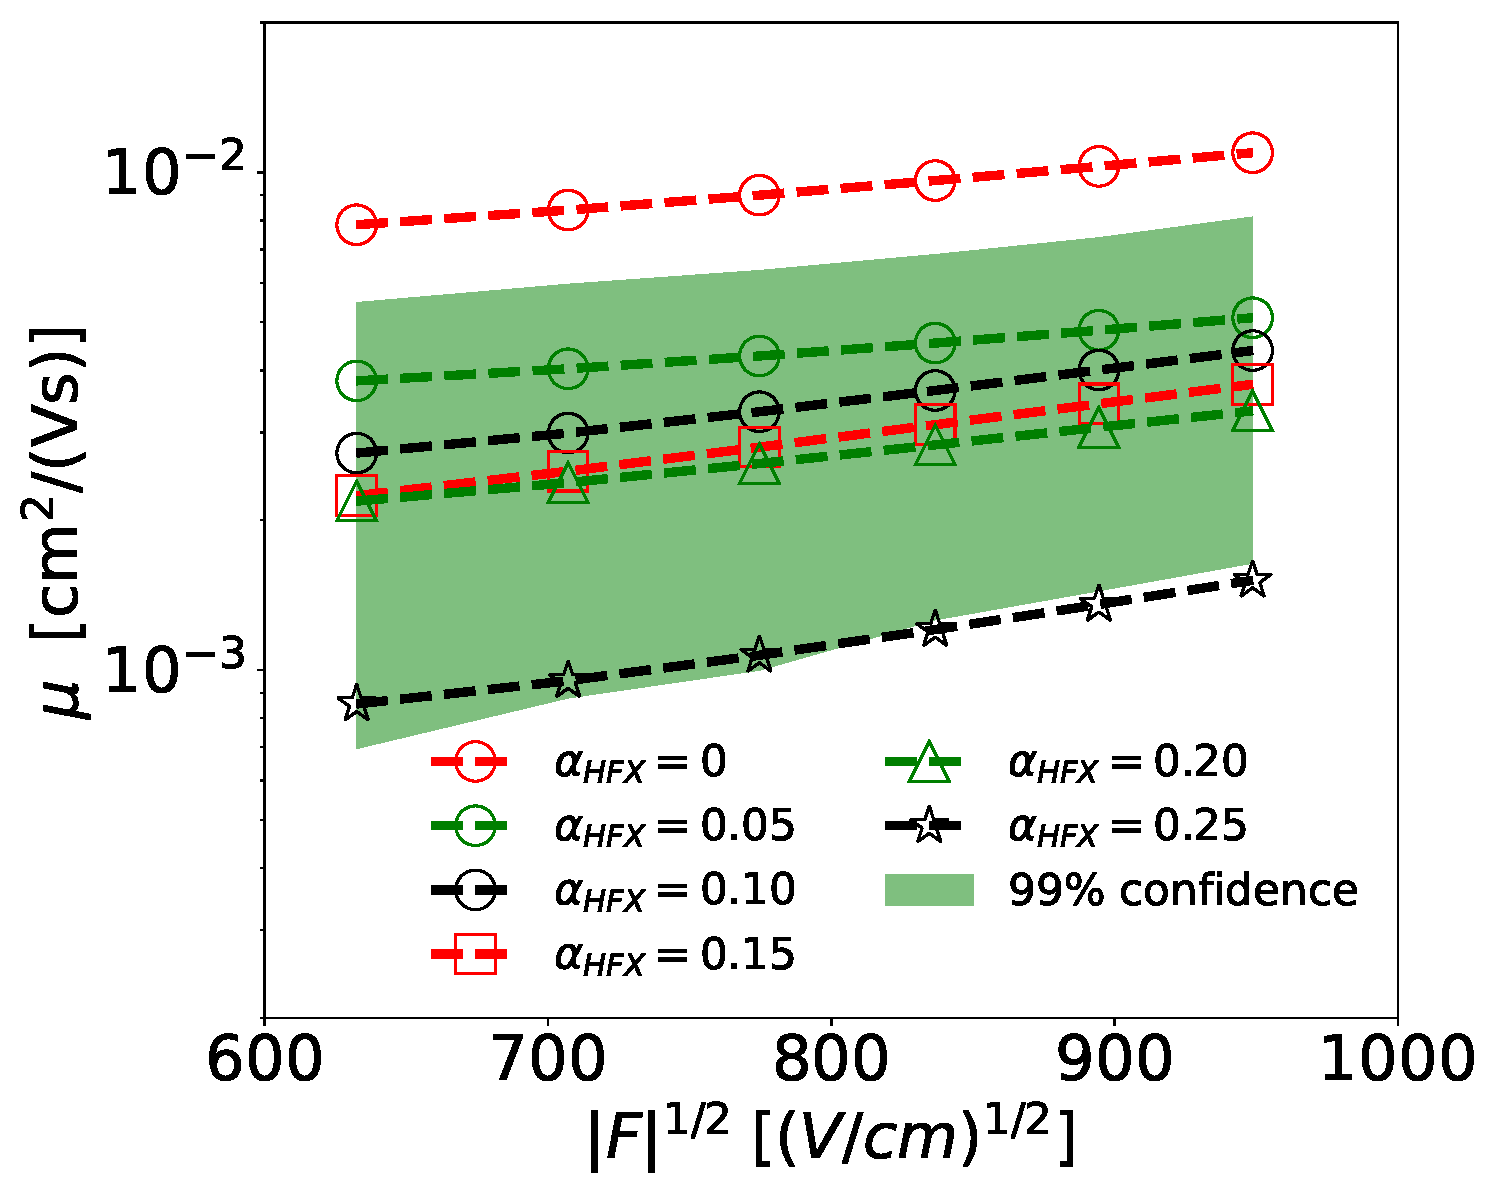
\includegraphics[width=0.45\textwidth]{figs/fig_PF_plot_ave.pdf}
    \caption{\bjoern{TODO Zhong:}{remove PF label; avoid the large white space at the right; make data plot symbols a little bigger and lines a little thicker.}Electric-field dependence of the mobility $\mu$ in the multiscale modeled MADN system. The dash lines are Poole–Frenkel plots obtained with specific HFX value, and the green shadow indicates the 99\% confidence interval estimated from the MC sampling with a sample size of $N_\text{MC}=10000$.}
    \label{fig:PF_plot_ave}
\end{figure}

%
\begin{table}[tbp]%The best place to locate the table environment is directly after its first reference in text
  \caption{\label{tab:PF_parameter}%
  Poole-Frenkel parameters $\mu_0$ (in $\unit[]{cm^2/(Vs)}$) and $\beta$ (in $\unit[]{\sqrt{cm/V}}$) of the multiscale modeled MADN, calculated by the six different HFX values. 
  }
  \begin{ruledtabular}
    \begin{tabular}{c c c c c}
    $\alpha$ & & $\mu_0$  & & $\beta$ \\
      \hline
    0 & & $4.0 \times 10^{-3}$ & & $1.0 \times 10^{-3}$ \\
    0.05 & & $2.1 \times 10^{-3}$ & & $9.3 \times 10^{-4}$ \\
    0.10 & & $1.0 \times 10^{-3}$ & & $1.5 \times 10^{-3}$ \\
    0.15 & & $8.0 \times 10^{-4}$ & & $1.6 \times 10^{-3}$ \\
    0.20 & & $9.3 \times 10^{-4}$ & & $1.3 \times 10^{-3}$ \\
    0.20 & & $2.6 \times 10^{-4}$ & & $1.8 \times 10^{-3}$ \\
      \end{tabular}
  \end{ruledtabular}
  \end{table}
%  
The extracted Poole–Frenkel paratermeter calculated from the six $\alpha$ values are summarized in Table \ref{tab:PF_parameter}. 
Excluding the data of $\alpha=0$, the extracted zero-field mobility $\mu_0$ has a range from $2.6 \times 10^{-4}$ to $2.1 \times 10^{-3}$, and the field effect constant $\beta$ range from $9.3 \times 10^{-4}$ to $1.8 \times 10^{-3}$.
So $\beta$ is less sensitive to the multiscale model parameter $\alpha$ compared the zero-field mobility.
%%%%%%%%%%%%%%%%%%%%%%%%%%%%%%%%%%%%%%%%%%%%%%%%%%%%%%%%%%%%%%%%%%%%
\section{Conclusion}
The uncertainty effect from the exchange-correlation functional of the DFT on the multiscale model of OSC is studied. By choosing different HFX, the calculated values of some electronic structures remain very similar,
such as the reorganization energy $\lambda$, molecular energy $E_i$ and the majority of the coupling elements  $J_{ij}$. While a few small-value coupling elements $J_{ij}$ show large different in calculated values when different HFX is used. Those uncertainties propagate to the output of the multiscale model, resulting in a range of QoI which has a maximum about 15 times of its minimum. These findings high-
light the importance of selecting appropriate functionals to ensure model robustness. Also indicated is that for multiscale model charge mobility, when the values have difference is approximately 10\%, we should interpret the results with caution and refrain from concluding that they represent fundamentally different phenomena.

Assuming the maximum amount of uncertainty from the calculated electronic structure parameters using the six HFX, the 99\% confidence level of the ToFs around the median are estimated. The Sobol indexes show that the molecular energy has the most contribution to the total variance, followed by the reorganization energy and coupling elements. Our results also shows that due to the uncertainties, the steady state velocity distribution spans 4 orders of magnitude. So it is less robust when
the electronic structure parameters are uncertain, and a useful range of velocity is hard to obtain. Future research should explore the impact of other sources of uncertainty and extend this framework to different types of semiconducting materials, thus enhancing the predictive power and applicability of multiscale models in the field.
% The \nocite command causes all entries in a bibliography to be printed out
% whether or not they are actually referenced in the text. This is appropriate
% for the sample file to show the different styles of references, but authors
% most likely will not want to use it.
%\nocite{*}

\bibliography{references}% Produces the bibliography via BibTeX.

\end{document}
%
% ****** End of file apssamp.tex ******
